% ==========================================================================
% CHAPTER 3 -- RESULTS AND DISCUSSION
%
% Presents what was obtained and explains what it means. All numbers are
% taken from the executed notebook outputs of the ASN manuscript study.
% ==========================================================================

\chapter{Results and Discussion}
\label{ch:results}

This chapter presents the results of the two evaluation protocols used in
this thesis and discusses their meaning. Section~\ref{sec:ch3_intro}
introduces the two protocols and their best-model results;
Section~\ref{sec:intra} reports the permissive intra-patient six-category
ECG study; Section~\ref{sec:inter} reports the record-disjoint inter-patient
five-class study, including the AAMI EC57 statistics, ablation analyses,
explainability, robustness, and microcontroller deployment;
Section~\ref{sec:crossprotocol} synthesises the two protocols; and
Section~\ref{sec:summary} closes with a summary of the findings.


\section{Introduction}
\label{sec:ch3_intro}

The proposed pipeline is evaluated under two deliberately different
protocols, and the contrast between them is itself one of the main themes of
this investigation. The first is an \emph{inter-patient}, record-disjoint
protocol based on the five ANSI/AAMI EC57 classes: normal (N),
supraventricular ectopic (S), ventricular ectopic (V), fusion (F), and
unknown/paced (Q)~\cite{aami_ec57_2012}, in which no patient contributes
beats to more than one partition. This is the regime under which arrhythmia
classifiers are comparable across studies, and it is much more difficult
because the model never sees a test patient during training. The second is
an \emph{intra-patient} protocol with a stratified train/validation/test
split and SMOTE balancing~\cite{chawla2002smote}, extended with a sixth
category comprising ECG segments derived from the BIDMC Congestive Heart
Failure Database (CHF). Because CHF is a cardiovascular clinical condition
rather than an ANSI/AAMI EC57 beat class, this arm is described throughout
as a six-\emph{category} ECG experiment rather than a six-class arrhythmia
problem; it is the more permissive, within-database regime frequently found
in the literature. The inter-patient protocol is the more stringent: it uses
a record-disjoint split so that no test patient's beats appear during
training, and it reports only the five AAMI EC57 classes. The intra-patient
protocol, by contrast, allows the same patient's beats in both training and
test partitions and adds a sixth, CHF-derived clinical-condition category.
The accuracy gap between the two arms---0.8945 versus 0.9859---quantifies
how much of the reported performance in the literature is an artefact of the
assessment regime rather than genuine generalisation.
Table~\ref{tab:protocols} compares the two protocols and their best-model
results. The intra-patient numbers cannot be compared with the inter-patient
numbers; the inter-patient protocol is the clinically meaningful one because
under a record-disjoint split none of the test patients' beats influenced
training.

\begin{table}[!t]
\centering
\caption{Comparison of the inter-patient (Part~A) and intra-patient (Part~B) evaluation protocols and their best-model results}
\label{tab:protocols}
\begin{tabular}{lcc}
\toprule
 & \textbf{Inter-patient (Part~A)} & \textbf{Intra-patient (Part~B)} \\
\midrule
Split                & record-disjoint          & stratified + SMOTE \\
Label set            & 5 AAMI classes (N/S/V/F/Q) & 5 + CHF-derived category \\
Balancing on test    & none                     & none \\
Test beats           & 9{,}112                  & 4{,}329 \\
Best accuracy        & 0.8945 (MSFT-Net)        & 0.9859 \\
Best macro-$F_1$     & 0.8725 (MSFT-Net)        & 0.9684 \\
\bottomrule
\end{tabular}
\end{table}

\section{Intra-Patient Six-Category Study}
\label{sec:intra}

The second protocol relaxes the record-disjoint constraint: a stratified
train/validation/test split is used, and a sixth category, comprising
R-peak-centred ECG segments derived from the BIDMC Congestive Heart Failure
Database, is added to the five AAMI beat categories to give a six-category
problem (N/S/V/F/Q plus a CHF-derived clinical-condition category)
evaluated on 4{,}329 test beats. This permissive, within-database regime is
widely used in the literature, and it is reported here both for completeness
and because its juxtaposition with the inter-patient results shows how much
apparent performance is a by-product of the assessment regime.

\subsection{Dataset Composition and Balancing}
\label{subsec:intra_data}

Beats were taken from the MIT-BIH Arrhythmia Database (48 records), the
MIT-BIH Normal Sinus Rhythm Database (18 records), which was mapped to the
normal class, and the BIDMC Congestive Heart Failure Database (15 records
at 250~Hz)~\cite{moody2001mitbih,goldberger2000physionet,baim1986chf}. The
normal and CHF contributions were each capped at 5{,}000 beats. Table
\ref{tab:intra_data} shows the composition from the raw extraction through
the normal-class cap to the SMOTE-balanced training set, and Figure
\ref{fig:intra_class_distribution} displays the raw imbalance.

\begin{table}[!t]
\centering
\caption[Composition of the intra-patient six-category ECG corpus]{Composition of the intra-patient six-category ECG corpus---five AAMI beat categories plus one CHF-derived clinical-condition category---from raw extraction through normal-class capping to the SMOTE-balanced training set}
\label{tab:intra_data}
\begin{tabular}{lrrr}
\toprule
\textbf{Class} & \textbf{Raw beats} & \textbf{After N-cap} & \textbf{Train (post-SMOTE)} \\
\midrule
N-Normal  & 10{,}000 & 5{,}000 & 5{,}627 \\
S-Supra   &  2{,}781 & 2{,}781 & 5{,}627 \\
V-Ventri  &  7{,}235 & 7{,}235 & 5{,}627 \\
F-Fusion  &    802  &    802  & 5{,}627 \\
Q-Unknown &  8{,}038 & 8{,}038 & 5{,}627 \\
CHF       &  5{,}000 & 5{,}000 & 5{,}627 \\
\midrule
Total     & 33{,}856 & 28{,}856 & 33{,}762 \\
\bottomrule
\end{tabular}
\end{table}

\begin{figure}[!t]
\centering
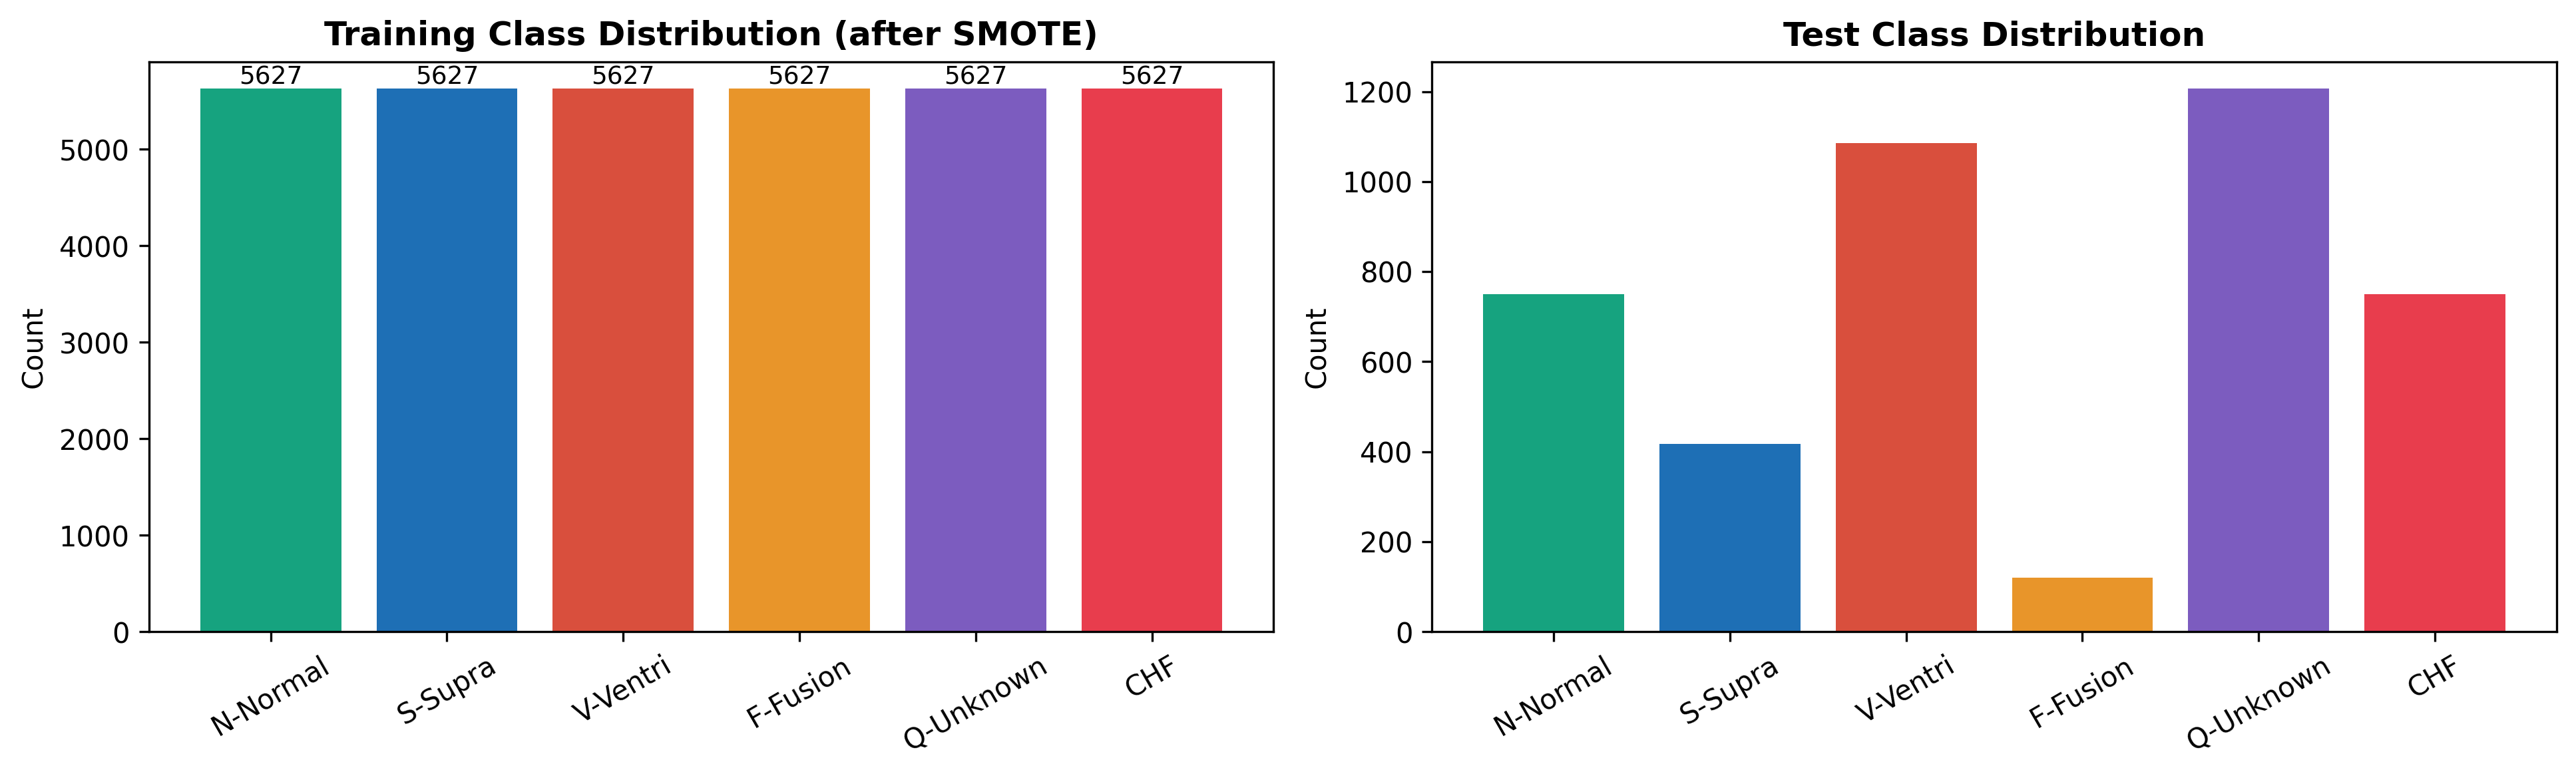
\includegraphics[width=0.95\linewidth]{figures/Intra_Patient/00_class_distribution.png}
\caption{Raw class distribution of the six-category intra-patient corpus before balancing}
\label{fig:intra_class_distribution}
\end{figure}

The data in Table~\ref{tab:intra_data} make two design decisions explicit.
Capping the normal class prevents the majority class from dominating the
SMOTE targets, and equalising the six training categories to 5{,}627 beats
avoids class imbalance as a confounding factor during optimisation. Both
choices are sensible for maximising within-database accuracy, but neither
concerns generalisation between patients, precisely because the split is
not record-disjoint, which is why the numbers below are substantially
higher than those of the inter-patient part.

\subsection{Training Dynamics and Overall Accuracy}
\label{subsec:intra_perf}

The CNN--BiLSTM--Attention model was trained for up to 50 epochs with early
stopping; Figure~\ref{fig:intra_training} shows how the learning curves
evolve. The overall test accuracy of the full model is 0.9859, with a
macro-$F_1$ of 0.9684. As Table~\ref{tab:intra_perclass} shows, five of the
six categories achieve $F_1$ scores of 0.96 or better; only the fusion class
remains difficult, with an $F_1$ of 0.84.

\begin{figure}[!t]
\centering
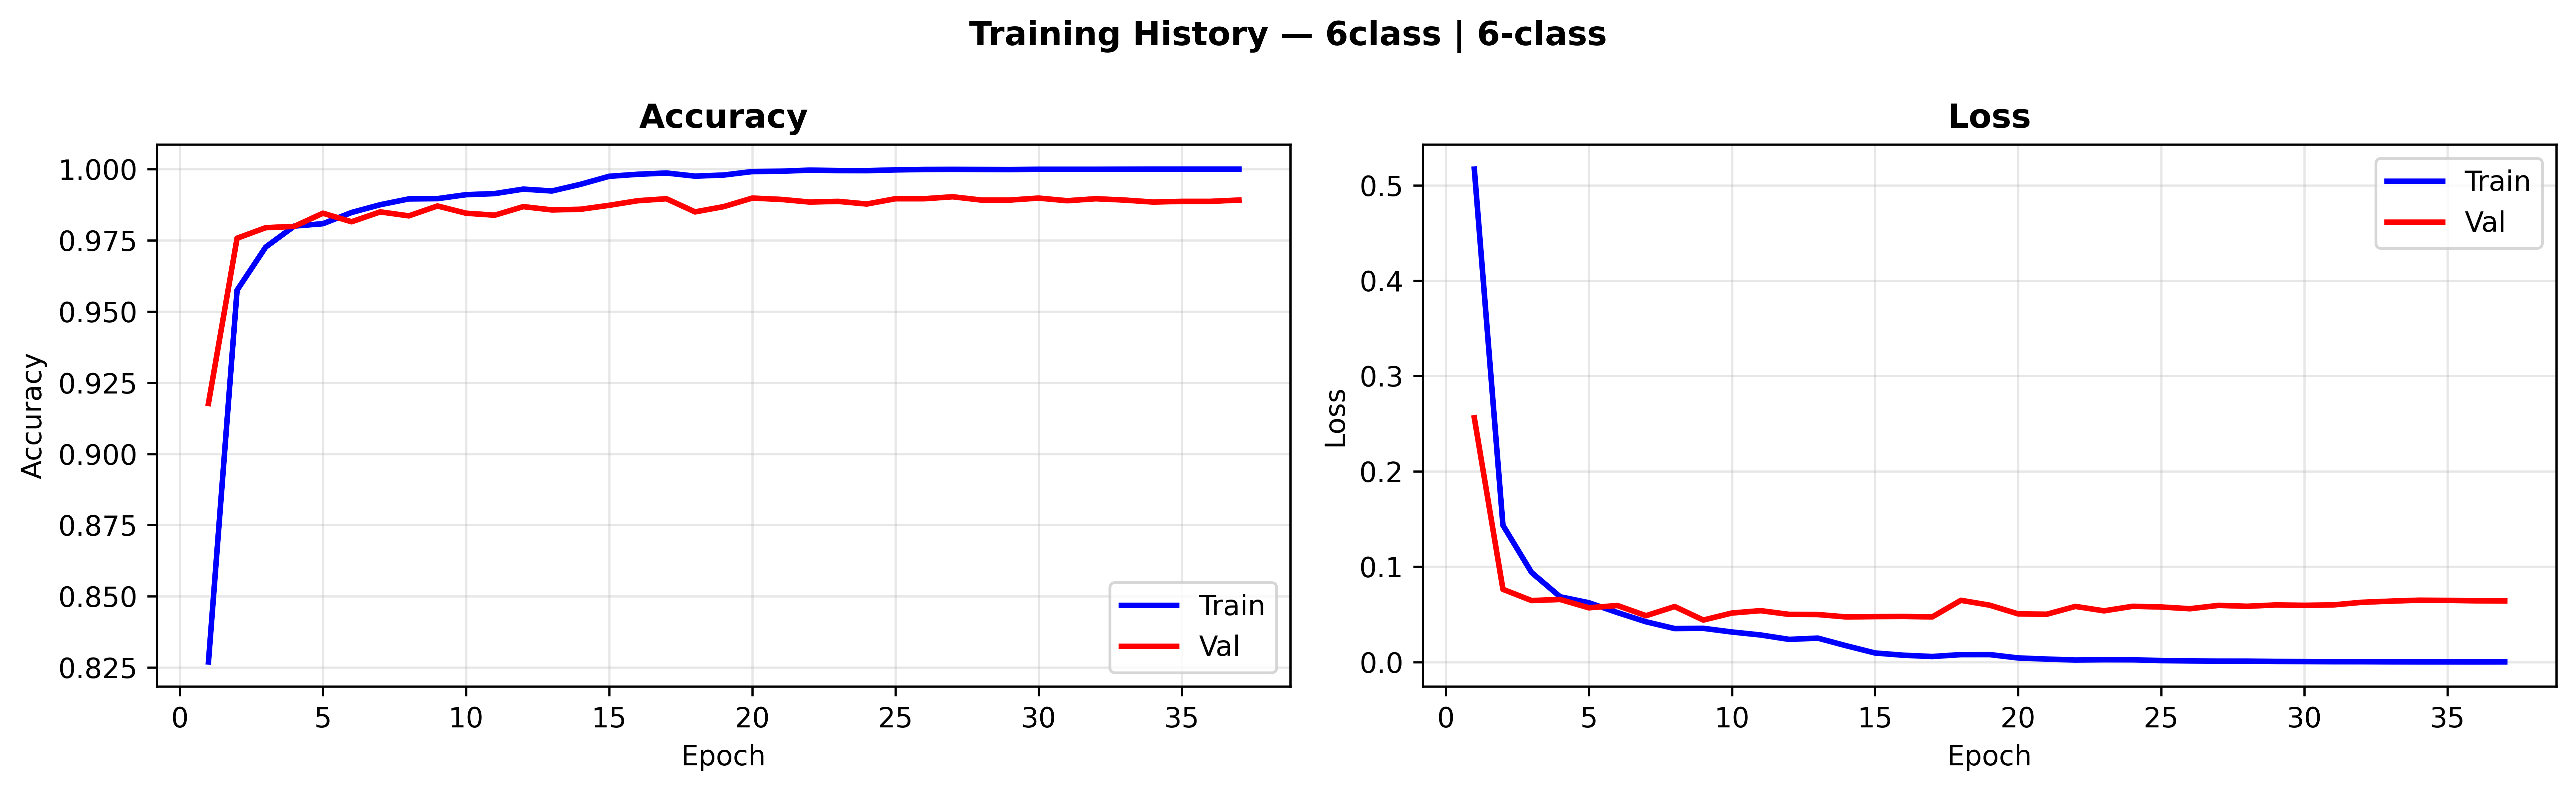
\includegraphics[width=0.95\linewidth]{figures/Intra_Patient/04_training_history.png}
\caption{Training and validation curves for the six-category hybrid under the intra-patient protocol}
\label{fig:intra_training}
\end{figure}

\begin{table}[!t]
\centering
\caption[Per-class precision, recall, and $F_1$ on the intra-patient six-category test set]{Per-class precision, recall, and $F_1$ on the intra-patient six-category test set (representative single-run report); CHF denotes the CHF-derived clinical-condition category}
\label{tab:intra_perclass}
\begin{tabular}{lrrrr}
\toprule
\textbf{Class} & \textbf{Precision} & \textbf{Recall} & \textbf{$F_1$} & \textbf{Support} \\
\midrule
N-Normal  & 0.99 & 1.00 & 0.99 & 750 \\
S-Supra   & 0.95 & 0.97 & 0.96 & 417 \\
V-Ventri  & 0.98 & 0.97 & 0.97 & 1{,}086 \\
F-Fusion  & 0.83 & 0.86 & 0.84 & 120 \\
Q-Unknown & 1.00 & 0.99 & 0.99 & 1{,}206 \\
CHF       & 1.00 & 0.99 & 0.99 & 750 \\
\midrule
Macro avg & 0.96 & 0.96 & 0.96 & 4{,}329 \\
Accuracy  & \multicolumn{3}{c}{0.9859} & 4{,}329 \\
\bottomrule
\end{tabular}
\end{table}

The CHF result must be interpreted with caution. As discussed in
Section~\ref{subsec:provenance}, the CHF segments come from a different
database with a different sampling frequency than the arrhythmia records, so
a large fraction of the model's CHF separability is likely due to a database
``fingerprint'' rather than cardiac morphology; it should not be read as
evidence of a clinically generalisable CHF signature. It is for this reason
that CHF was excluded from the rigorous five-class study. The one class that
remains difficult even under the permissive protocol is fusion: its $F_1$ of
0.84 even when training and test patients coincide is evidence that the
fusion difficulty is genuinely morphological, not an artefact of the
record-disjoint split, and it retrospectively validates the dedicated
fusion-handling pipeline of Section~\ref{subsec:fbeat}.

\subsection{Confusion Structure and ROC}
\label{subsec:intra_cm}

Figures~\ref{fig:intra_cm} and~\ref{fig:intra_roc} present the six-category
confusion matrix and the one-versus-rest ROC curves. The residual error is
concentrated in the fusion row and column, mirroring the inter-patient
finding that fusion is the binding constraint on performance. The ROC curves
are practically saturated, which is the logical result of a subject-mixed
split: at test time the model has already seen the typical waveform of each
patient, so detecting that patient's beat types is a much simpler problem
than picking out beat types on a patient it has never seen. This is the
quantitative centre of the cross-protocol comparison in
Section~\ref{sec:crossprotocol}.

\begin{figure}[!t]
\centering
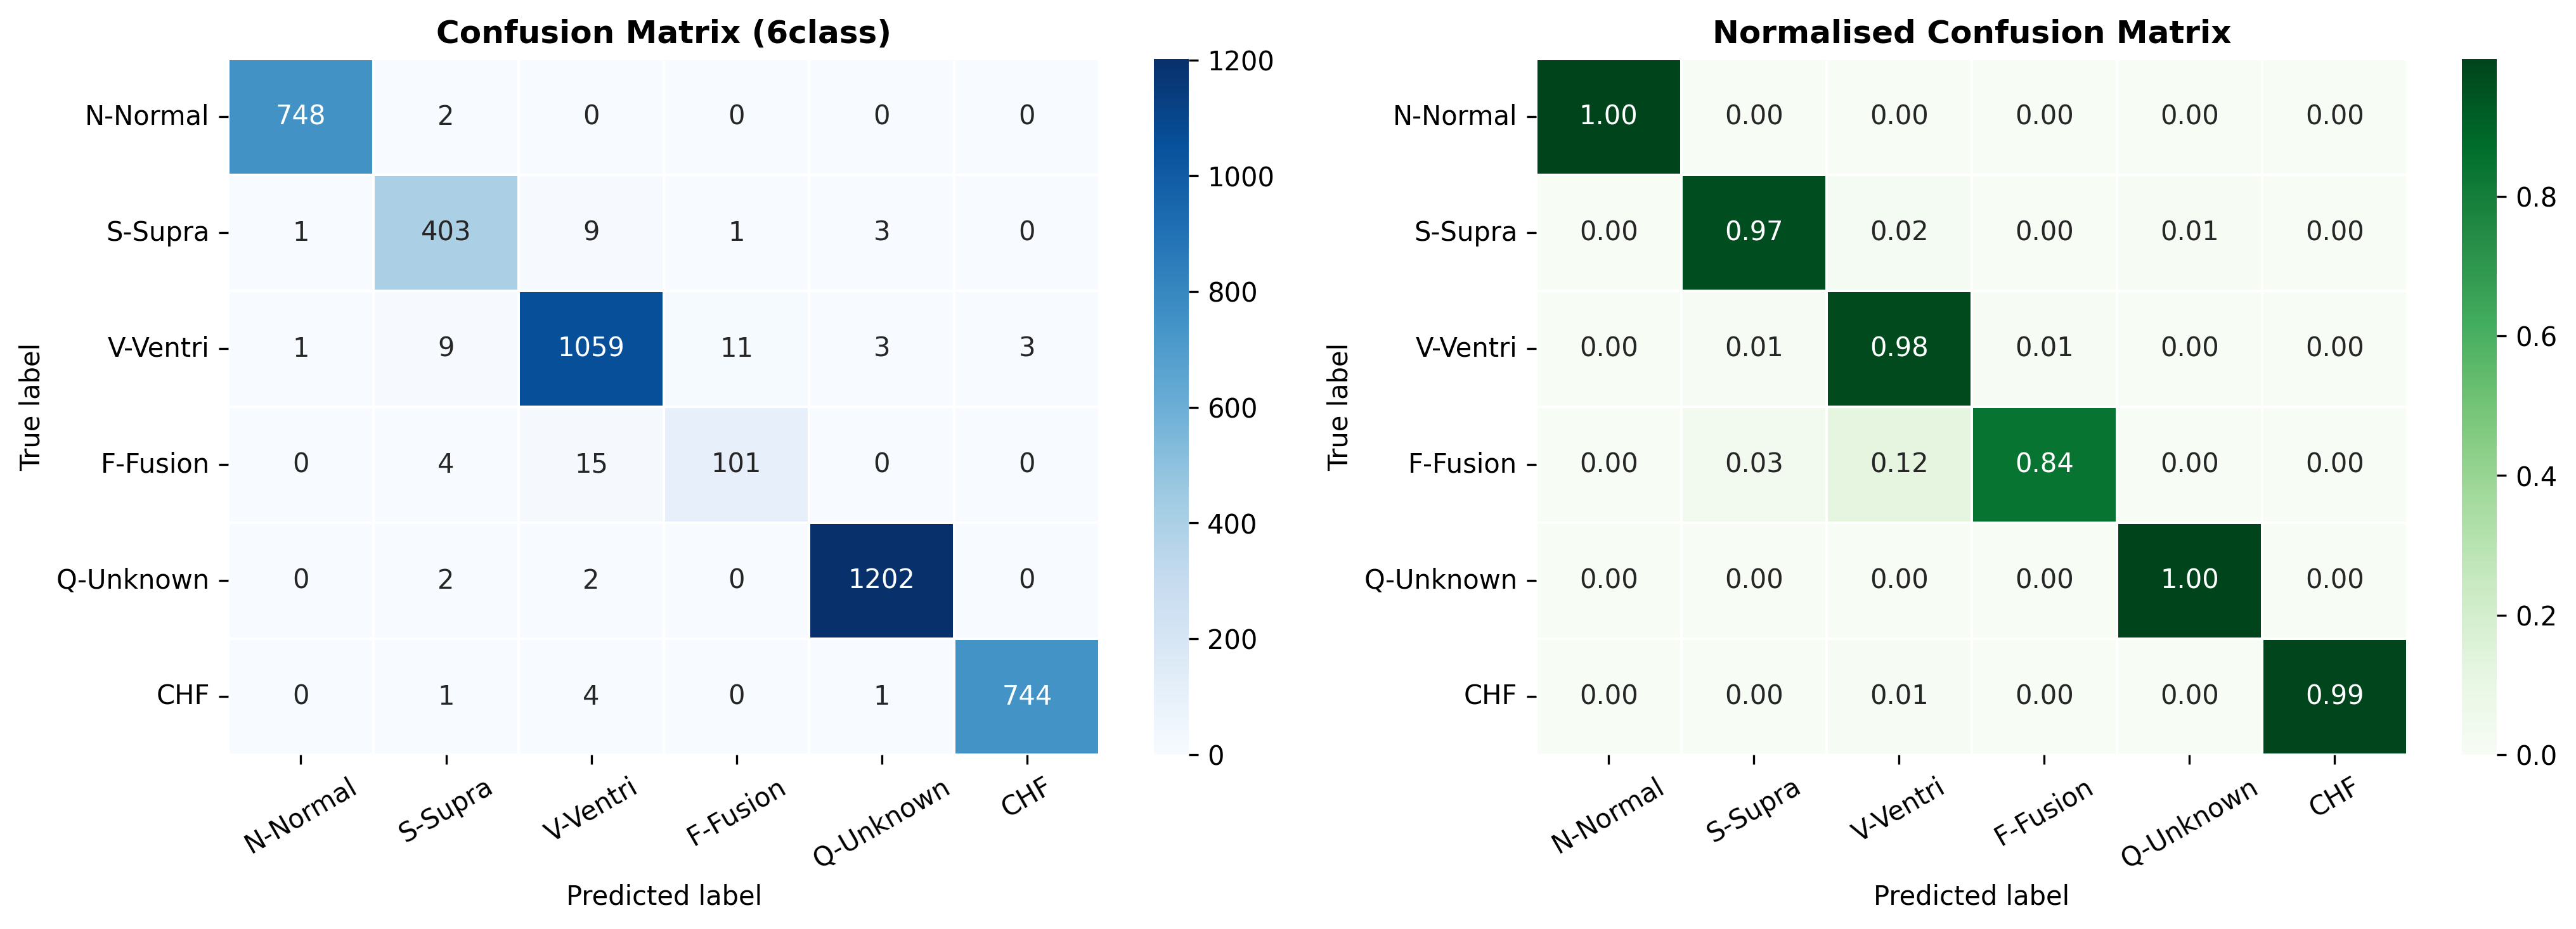
\includegraphics[width=0.95\linewidth]{figures/Intra_Patient/02_confusion_matrix.png}
\caption{Confusion matrix for the six-category intra-patient ECG classification experiment}
\label{fig:intra_cm}
\end{figure}

\begin{figure}[!t]
\centering
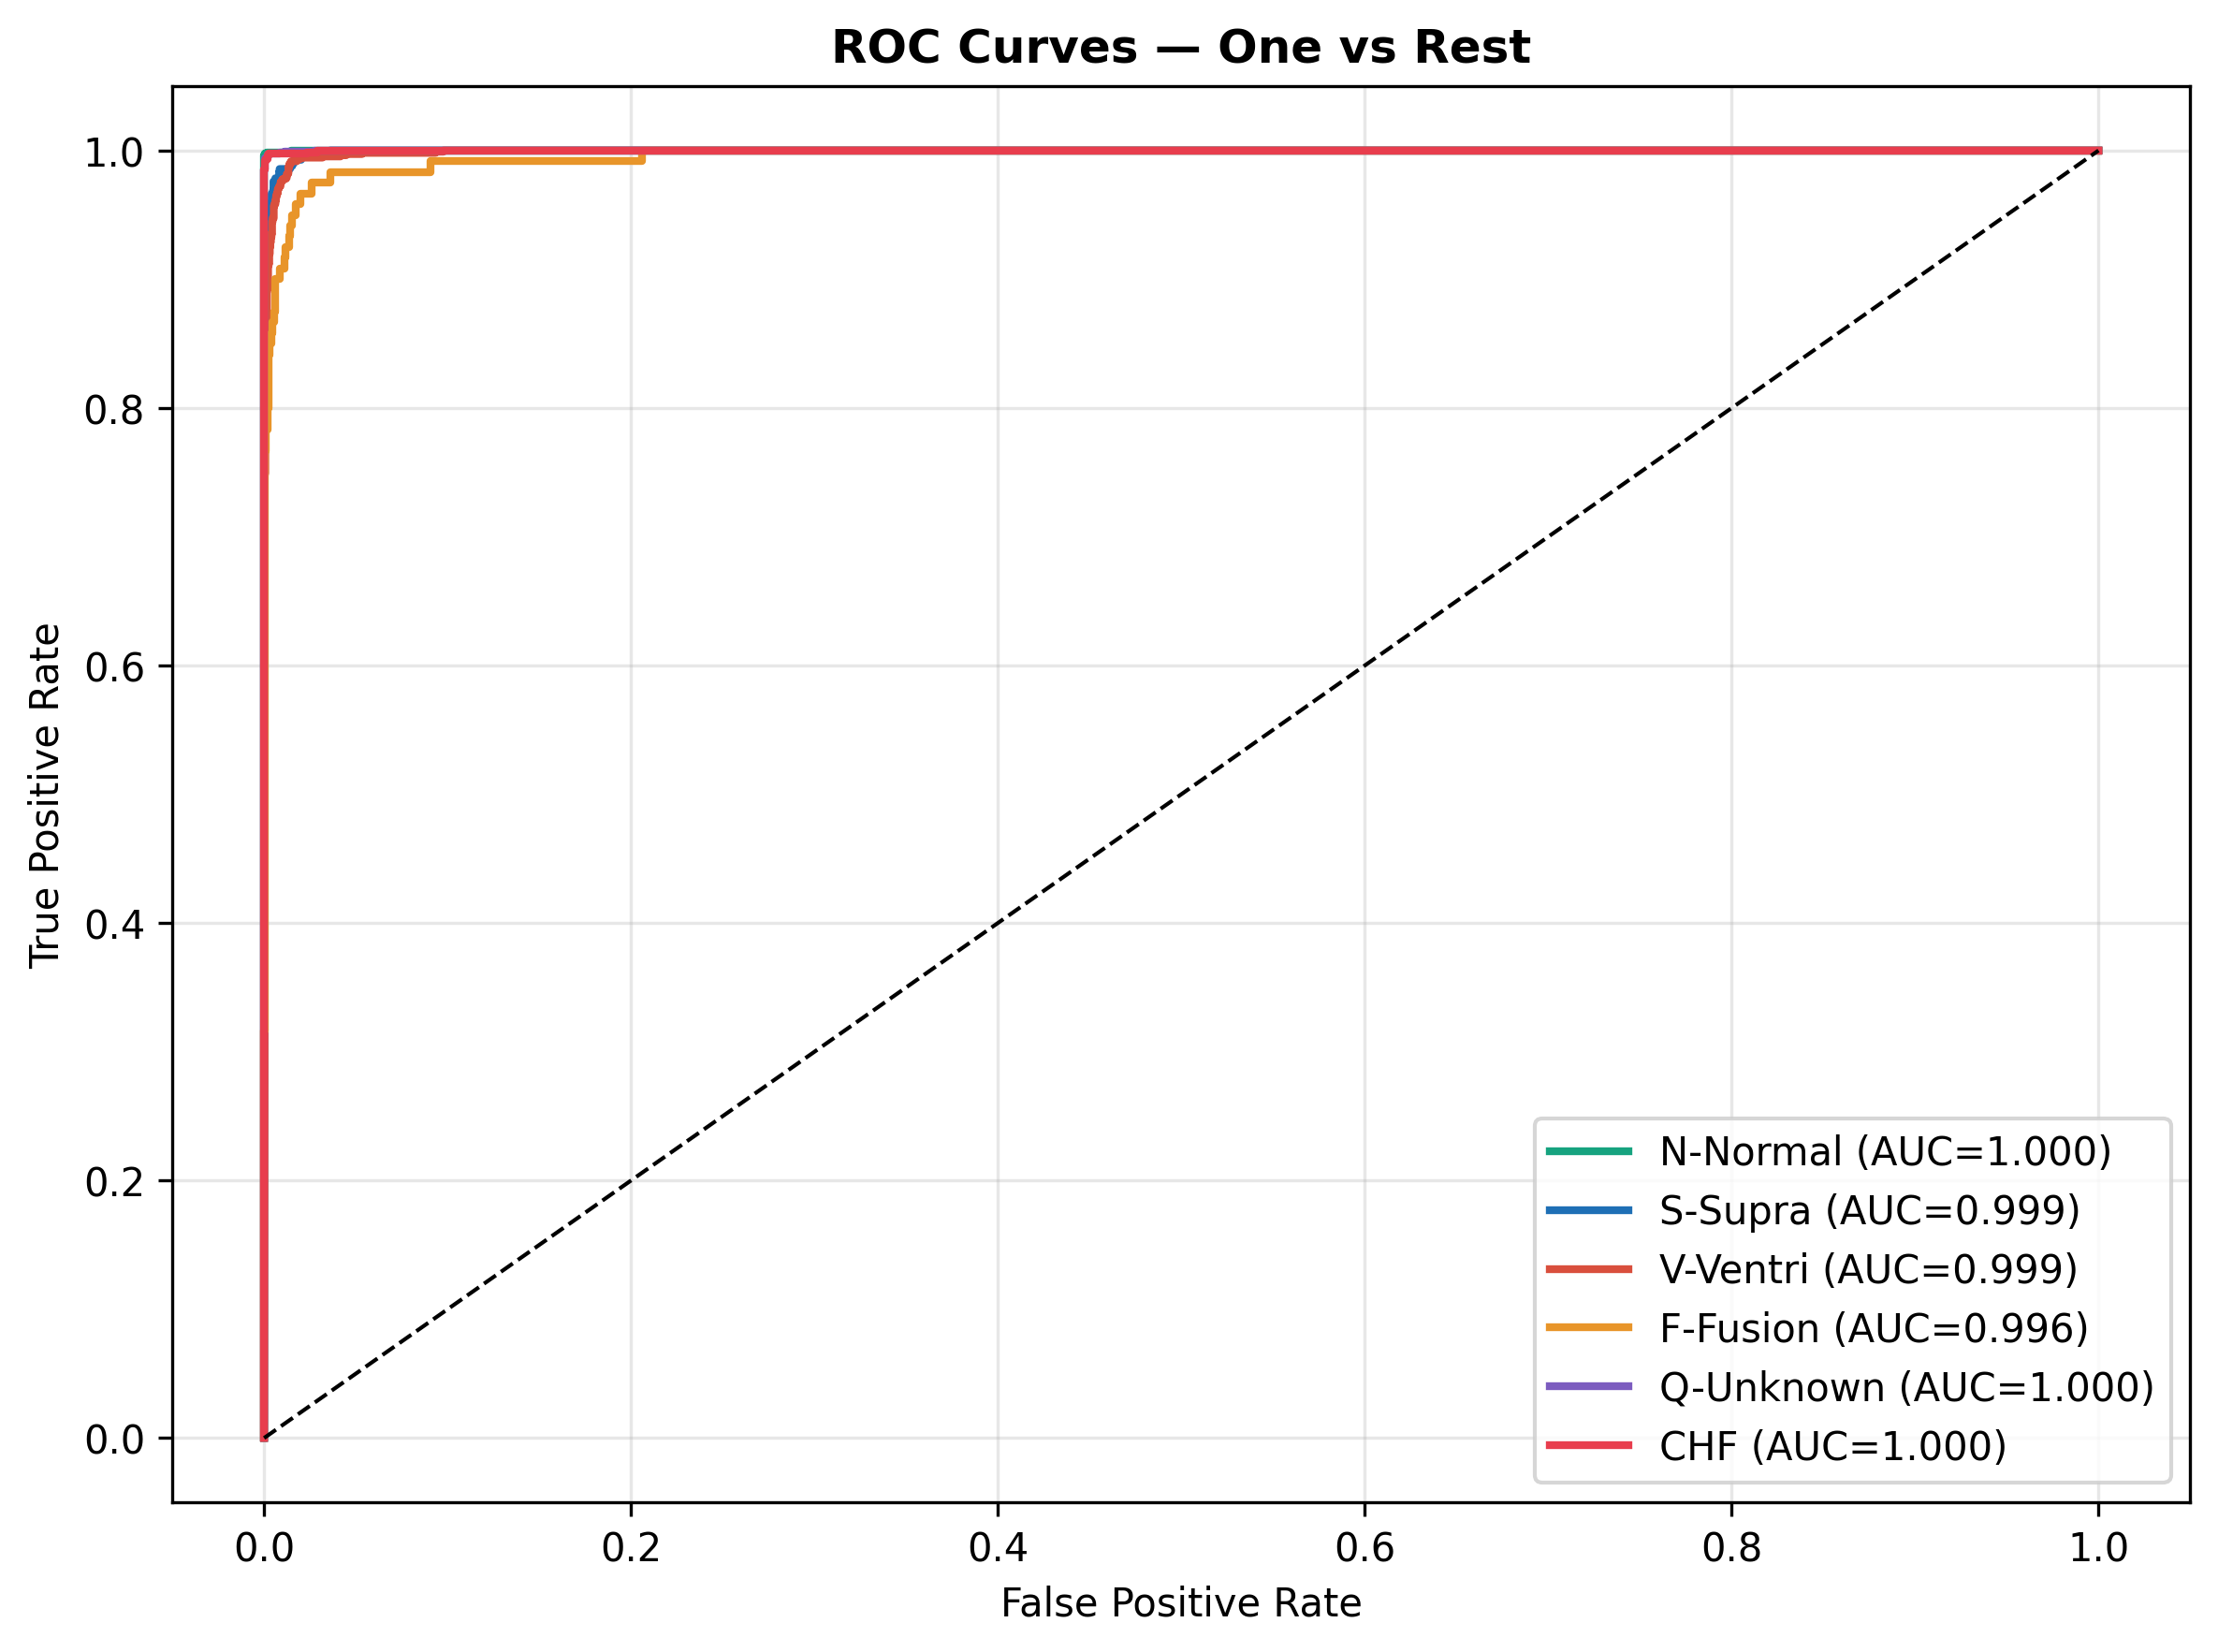
\includegraphics[width=0.75\linewidth]{figures/Intra_Patient/03_roc_curves.png}
\caption{One-versus-rest ROC curves for the six-category intra-patient ECG classification experiment}
\label{fig:intra_roc}
\end{figure}

\subsection{Ablation: Contribution of the Recurrent and Attention Stages}
\label{subsec:intra_ablation}

Table~\ref{tab:intra_ablation} and Figure~\ref{fig:intra_ablation} isolate
the contribution of the BiLSTM and attention stages by progressively
building the architecture from a CNN-only baseline.

\begin{table}[!t]
\centering
\caption{Architecture ablation under the intra-patient protocol}
\label{tab:intra_ablation}
\begin{tabular}{lrrr}
\toprule
\textbf{Model} & \textbf{Accuracy} & \textbf{Macro-$F_1$} & \textbf{$\Delta$Acc} \\
\midrule
CNN only                            & 0.9799 & 0.9604 & -- \\
CNN + BiLSTM                        & 0.9843 & 0.9660 & $+0.0044$ \\
CNN + BiLSTM + Attention (proposed) & 0.9834 & 0.9649 & $+0.0035$ \\
\bottomrule
\end{tabular}
\end{table}

\begin{figure}[!t]
\centering
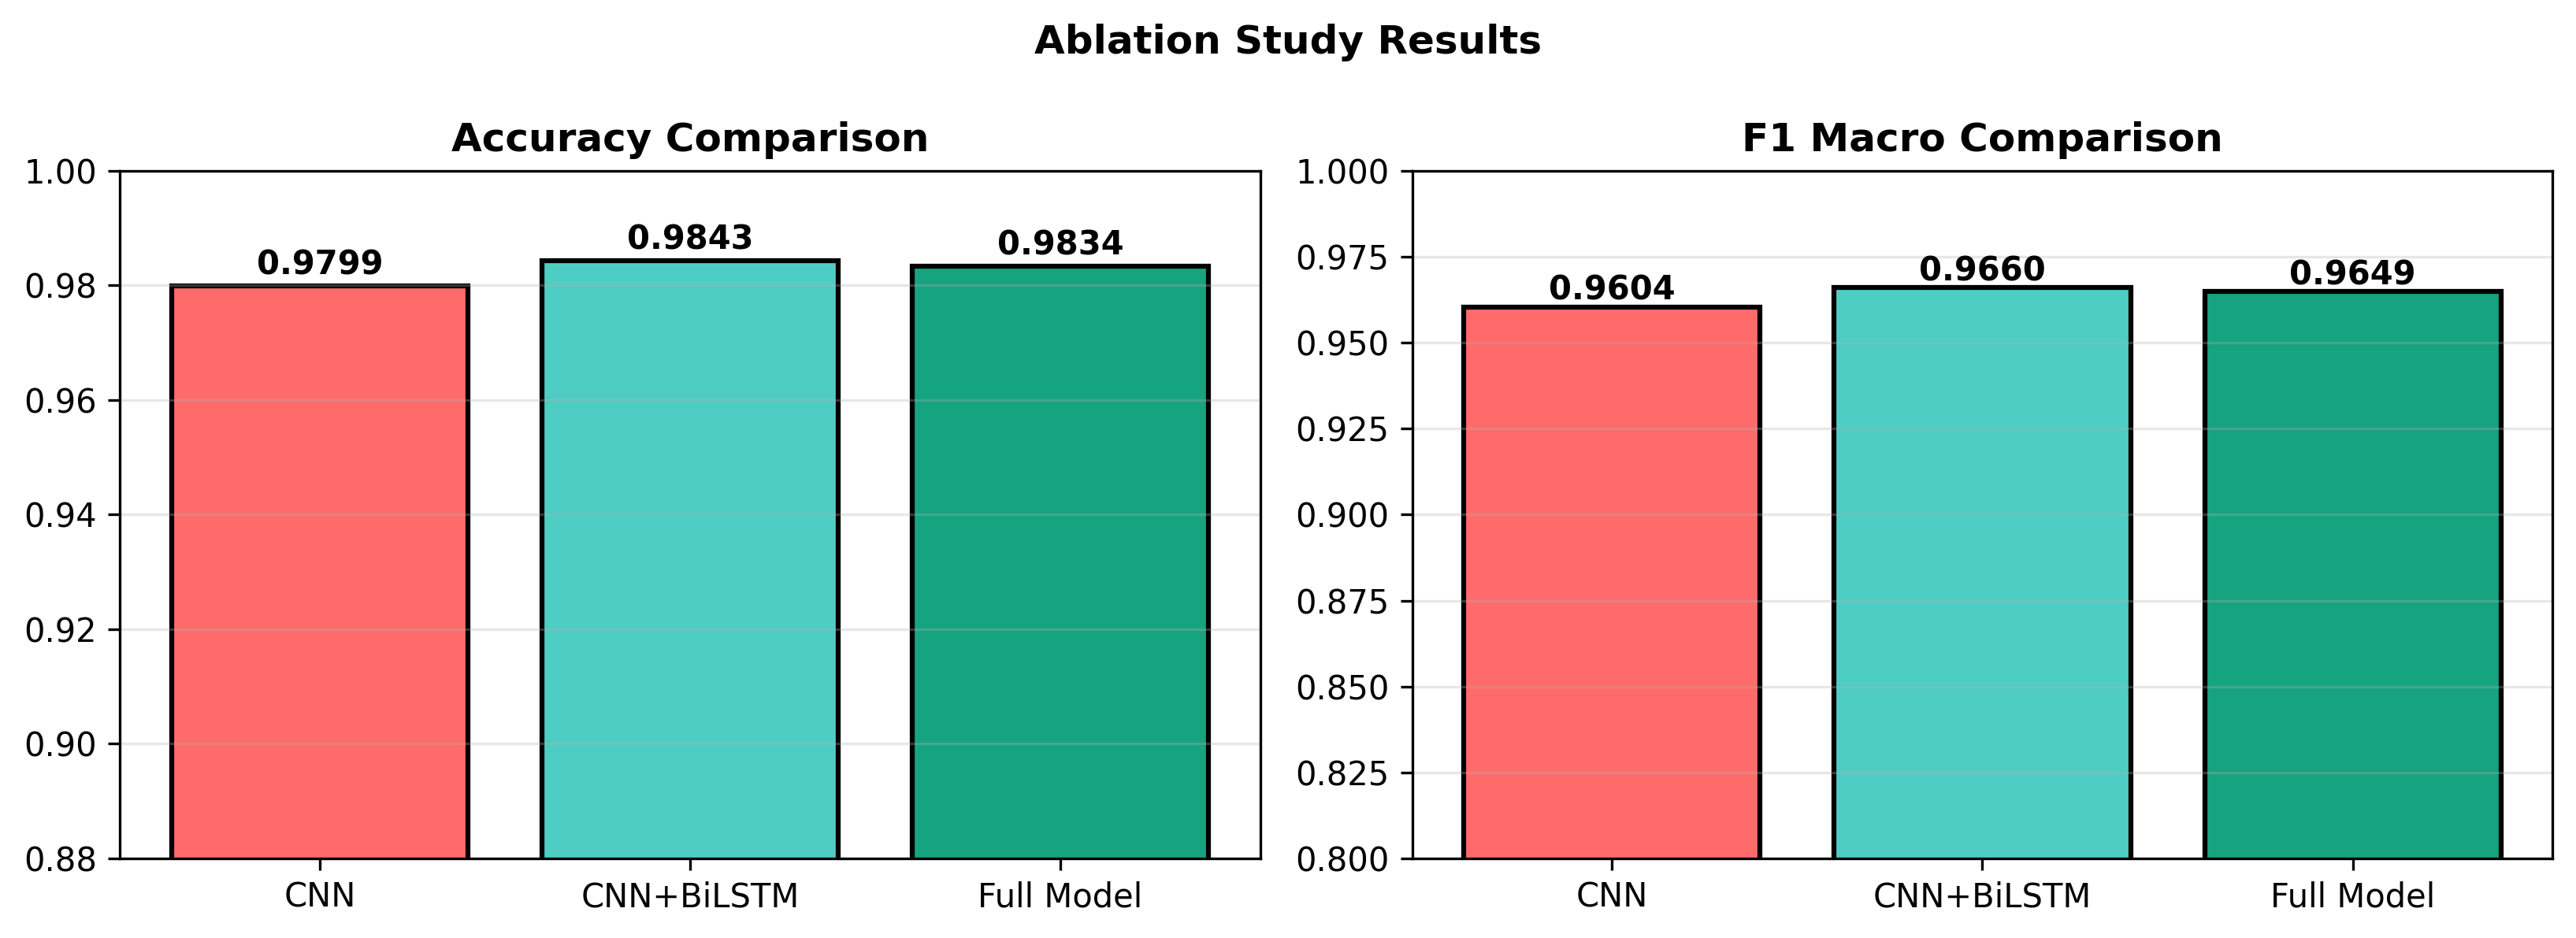
\includegraphics[width=0.95\linewidth]{figures/Intra_Patient/05_ablation.png}
\caption{Accuracy and macro-$F_1$ across the three architecture arms under the intra-patient protocol}
\label{fig:intra_ablation}
\end{figure}

Table~\ref{tab:intra_ablation} contains an instructive result that directly
contradicts what will be found under the record-disjoint split: the BiLSTM
stage contributes a measurable accuracy gain of 0.0044 (and a macro-$F_1$
gain of 0.0056) under the subject-mixed
split, while the attention stage adds nothing further (accuracy in fact
decreases by 0.0009). The recurrent stage exploits patient-dependent temporal regularities
that are present in a subject-mixed split but absent, by design, from the
held-out patients of a record-disjoint split. In other words, part of what
the recurrent stage learns is not transferable arrhythmia morphology but
patient identity. This is a concrete, data-based demonstration of why the
evaluation protocol changes not only the numbers reported but also the
architectural conclusions drawn from them.

\subsection{Model Compression}
\label{subsec:intra_compress}

The six-category hybrid was also compressed for edge deployment. Dynamic-range
quantisation reduced the converted lightweight model from 1.21~MB to
0.14~MB, an 88.42\% reduction, but the measured test accuracy dropped to
0.1737, just above the 0.167 chance level for the six-way problem. The dynamic-range
conversion, applied without a representative calibration data set, did not
maintain the decision function. This is reported as an intentional negative
result: it contrasts with the inter-patient INT8 model of
Section~\ref{subsec:mcu}, which was quantised with proper post-training
integer calibration. The practical lesson is that aggressive compression is
feasible only when faithful low-bit quantisation is performed with
appropriate calibration data, not by dynamic-range conversion alone.

\subsection{Comparison with Reported Methods}
\label{subsec:intra_sota}

Table~\ref{tab:sota} restates the comparison found in the executed
notebook, comparing the intra-patient six-category model against representative
reported ECG-classification methods. Because the studies are based on
different databases, class groupings, and, most importantly, different
train/test protocols, the comparison is indicative only; the numbers are
not to be read as a like-for-like ranking.

\begin{table}[!t]
\centering
\caption{Indicative comparison of the intra-patient six-category model with reported ECG-classification methods}
\label{tab:sota}
\setlength{\tabcolsep}{3.5pt}%
\begin{tabular}{@{}>{\raggedright\arraybackslash}p{1.7in}>{\raggedright\arraybackslash}p{1.7in}ccc@{}}
\toprule
\textbf{Method} & \textbf{Dataset} & \textbf{Categories} & \textbf{Accuracy} & \textbf{Macro-$F_1$} \\
\midrule
This work\newline(CNN+BiLSTM+Att.\ +XAI) & MIT-BIH+NSR+CHF & 6 & 0.9859 & 0.9684 \\
CNN--BiLSTM+Att                 & MIT-BIH         & 5 & 0.9920 & 0.9750 \\
CNN+LSTM+Att                    & MIT-BIH+PTB     & 5 & 0.9930 & 0.9600 \\
Transformer ECG                 & MIT-BIH         & 5 & 0.9832 & 0.9501 \\
DenseNet1D                      & MIT-BIH         & 5 & 0.9756 & 0.9234 \\
LSTM--FCN                       & MIT-BIH         & 5 & 0.9634 & 0.8967 \\
SVM baseline                    & MIT-BIH         & 5 & 0.8976 & 0.7832 \\
\bottomrule
\end{tabular}
\end{table}

Table~\ref{tab:sota} puts the intra-patient model in perspective: it
achieves roughly the same performance as recent deep learning approaches,
with two characteristics that most of them lack: a six-category label set
that adds a CHF-derived category, and multi-database training. The most honest
interpretation of this table, however, is comparative rather than
competitive: several listed methods report slightly higher accuracy on the
narrower five-class MIT-BIH problem, and none of the external numbers was
obtained under a record-disjoint protocol. The results of
Section~\ref{sec:inter} show that Part~A is the more challenging and
clinically important test, so the meaning of the present work is not to sit
at the head of this table but to report both protocols transparently so
that apparent performance differences can be attributed to their real
source.


\section{Inter-Patient (Record-Disjoint) Five-Class Study}
\label{sec:inter}

All metrics in this section are calculated on a frozen inter-patient test
partition of 9{,}112 beats from 26 patients of the MIT-BIH Arrhythmia
Database~\cite{moody2001mitbih,goldberger2000physionet}.

\subsection{Dataset Composition and Partitioning}
\label{subsec:dataset}

The beat corpus was assembled from three source types: 48 MIT-BIH records
covering multiple rhythms, 18 MIT-BIH Normal Sinus Rhythm records used to
augment the normal class, and a congestive-heart-failure set that was not
included in the final label space following the provenance controls of
Section~\ref{subsec:provenance}. To keep the study EC57-conformant, the four
paced records (102, 104, 107, 217) contribute $Q$ beats only, so that the
N/S/V/F supports are equivalent to a paced-free run. Table~\ref{tab:dataset}
summarises the class-wise beat counts, the record-disjoint split, and the
record coverage; the resulting class imbalance is visualised in
Figure~\ref{fig:class_distribution}. Two consequences of the sampling rules
deserve emphasis. First, because the per-record quotas of
Section~\ref{sec:proposed_methodology} preserve every available $S$ and $F$
beat, the $S$ and $F$ totals equal their complete raw populations (2,781 and
802 beats, identical to the raw extraction of Section~\ref{subsec:intra_data}),
whereas the abundant $N$, $V$, and $Q$ classes are bounded by the quotas.
The comparatively small $V$ total (667 beats) therefore reflects quota
sampling rather than the underlying prevalence of ventricular ectopy, and
the per-class test supports should be read in this light.

\begin{table}[!t]
\centering
\caption{Beat-level composition of the five AAMI classes and the record-disjoint partitioning}
\label{tab:dataset}
\begin{tabular}{lrrrrr}
\toprule
\textbf{Class} & \textbf{Records} & \textbf{Total beats} & \textbf{Train} & \textbf{Val.} & \textbf{Test} \\
\midrule
N-Normal   & 58 & 15{,}306 & 7{,}455 & 1{,}804 & 6{,}047 \\
S-Supra    & 32 &  2{,}781 &   774   &   170   & 1{,}837 \\
V-Ventri   & 25 &    667   &   283   &    51   &   333   \\
F-Fusion   & 17 &    802   &   399   &    15   &   388   \\
Q-Unknown  &  9 &  2{,}015 & 1{,}008 &   500   &   507   \\
\midrule
Total      & -- & 21{,}571 & 9{,}919 & 2{,}540 & 9{,}112 \\
\bottomrule
\end{tabular}
\end{table}

\begin{figure}[!t]
\centering
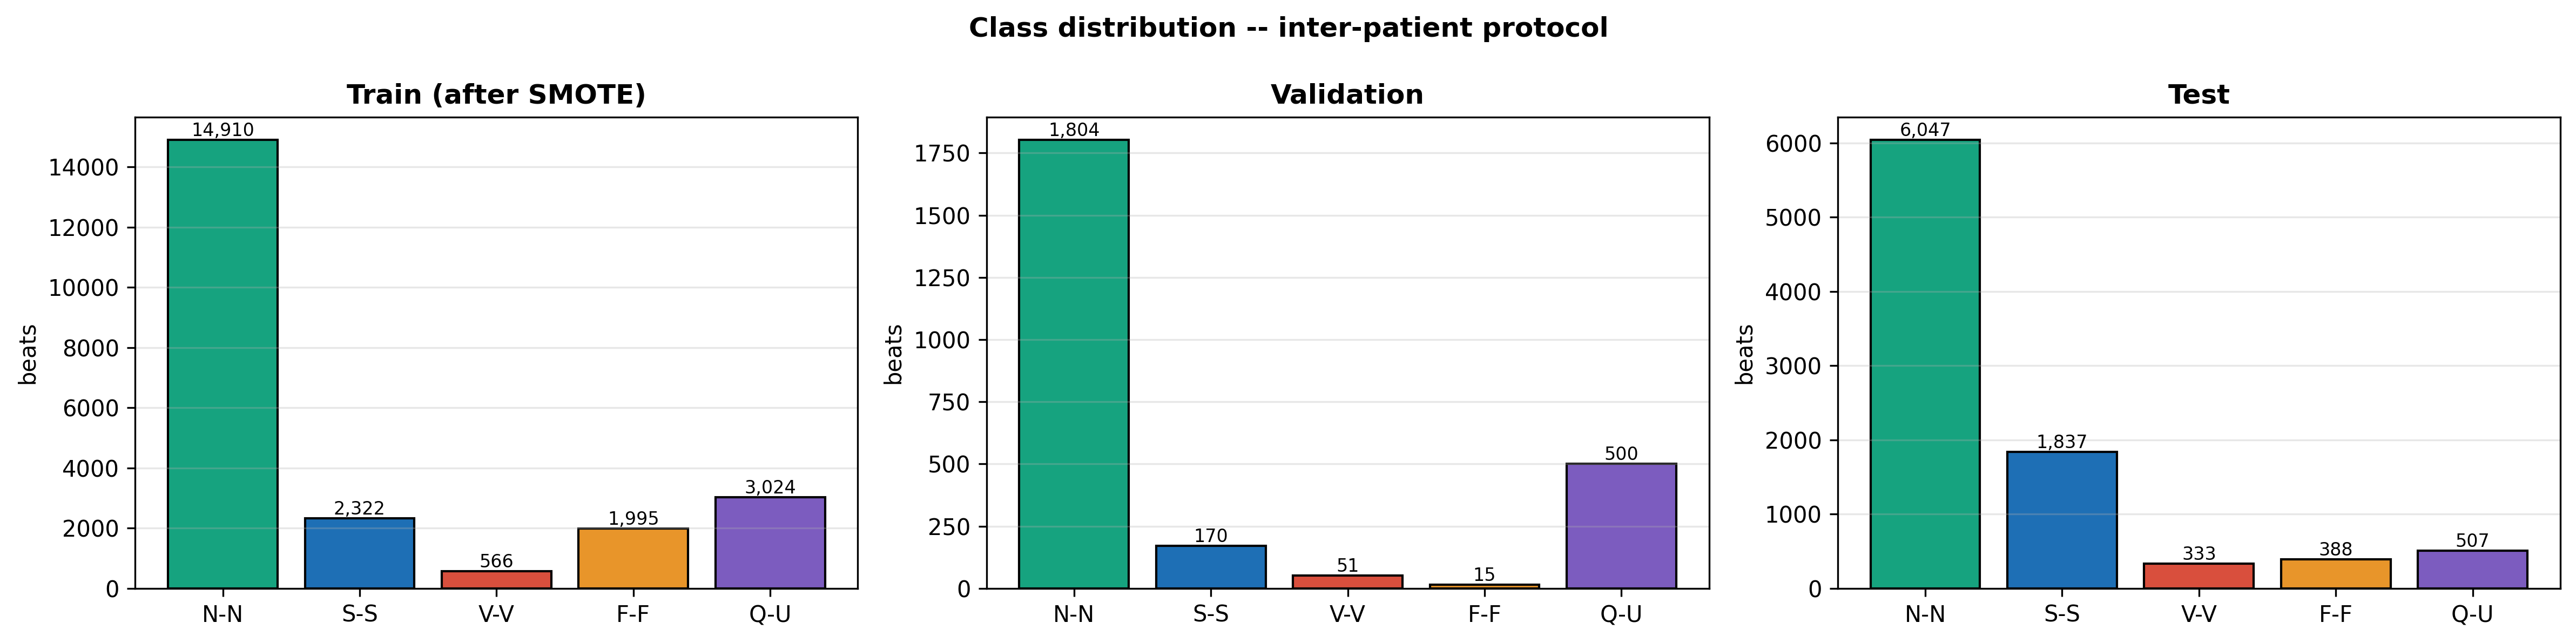
\includegraphics[width=0.95\linewidth]{figures/Inter_Patient/00_class_distribution.png}
\caption{Class distribution of the assembled beat corpus under the inter-patient protocol}
\label{fig:class_distribution}
\end{figure}

The class distribution in Figure~\ref{fig:class_distribution} is strongly
imbalanced and clinically representative: fusion and ventricular beats
occur rarely, yet they are the most expensive to miss when diagnosing.
Training-only augmentation was applied to the minority classes (one
perturbed copy of every training $S$ beat and three additional copies of
every training $F$ beat), adding 1{,}971 beats and expanding the training
set from 9{,}919 to 11{,}890
beats, while validation and test partitions were left untouched. The RR
timing, QRS morphology, wavelet descriptors, and N/V-template-similarity
features were computed from training statistics only, without using
validation or test labels, so the scale of any feature or template cannot
be contaminated by test information.

\subsection{Training Dynamics}
\label{subsec:training}

Figures~\ref{fig:train_hybrid} and~\ref{fig:train_msft} show the learning
curves of the two architectures: the CNN--BiLSTM--Attention hybrid (572{,}358
parameters) and the lighter MSFT-Net (167{,}090 parameters) with multi-scale
convolutions, squeeze-and-excitation, and FiLM conditioning.

\begin{figure}[!t]
\centering
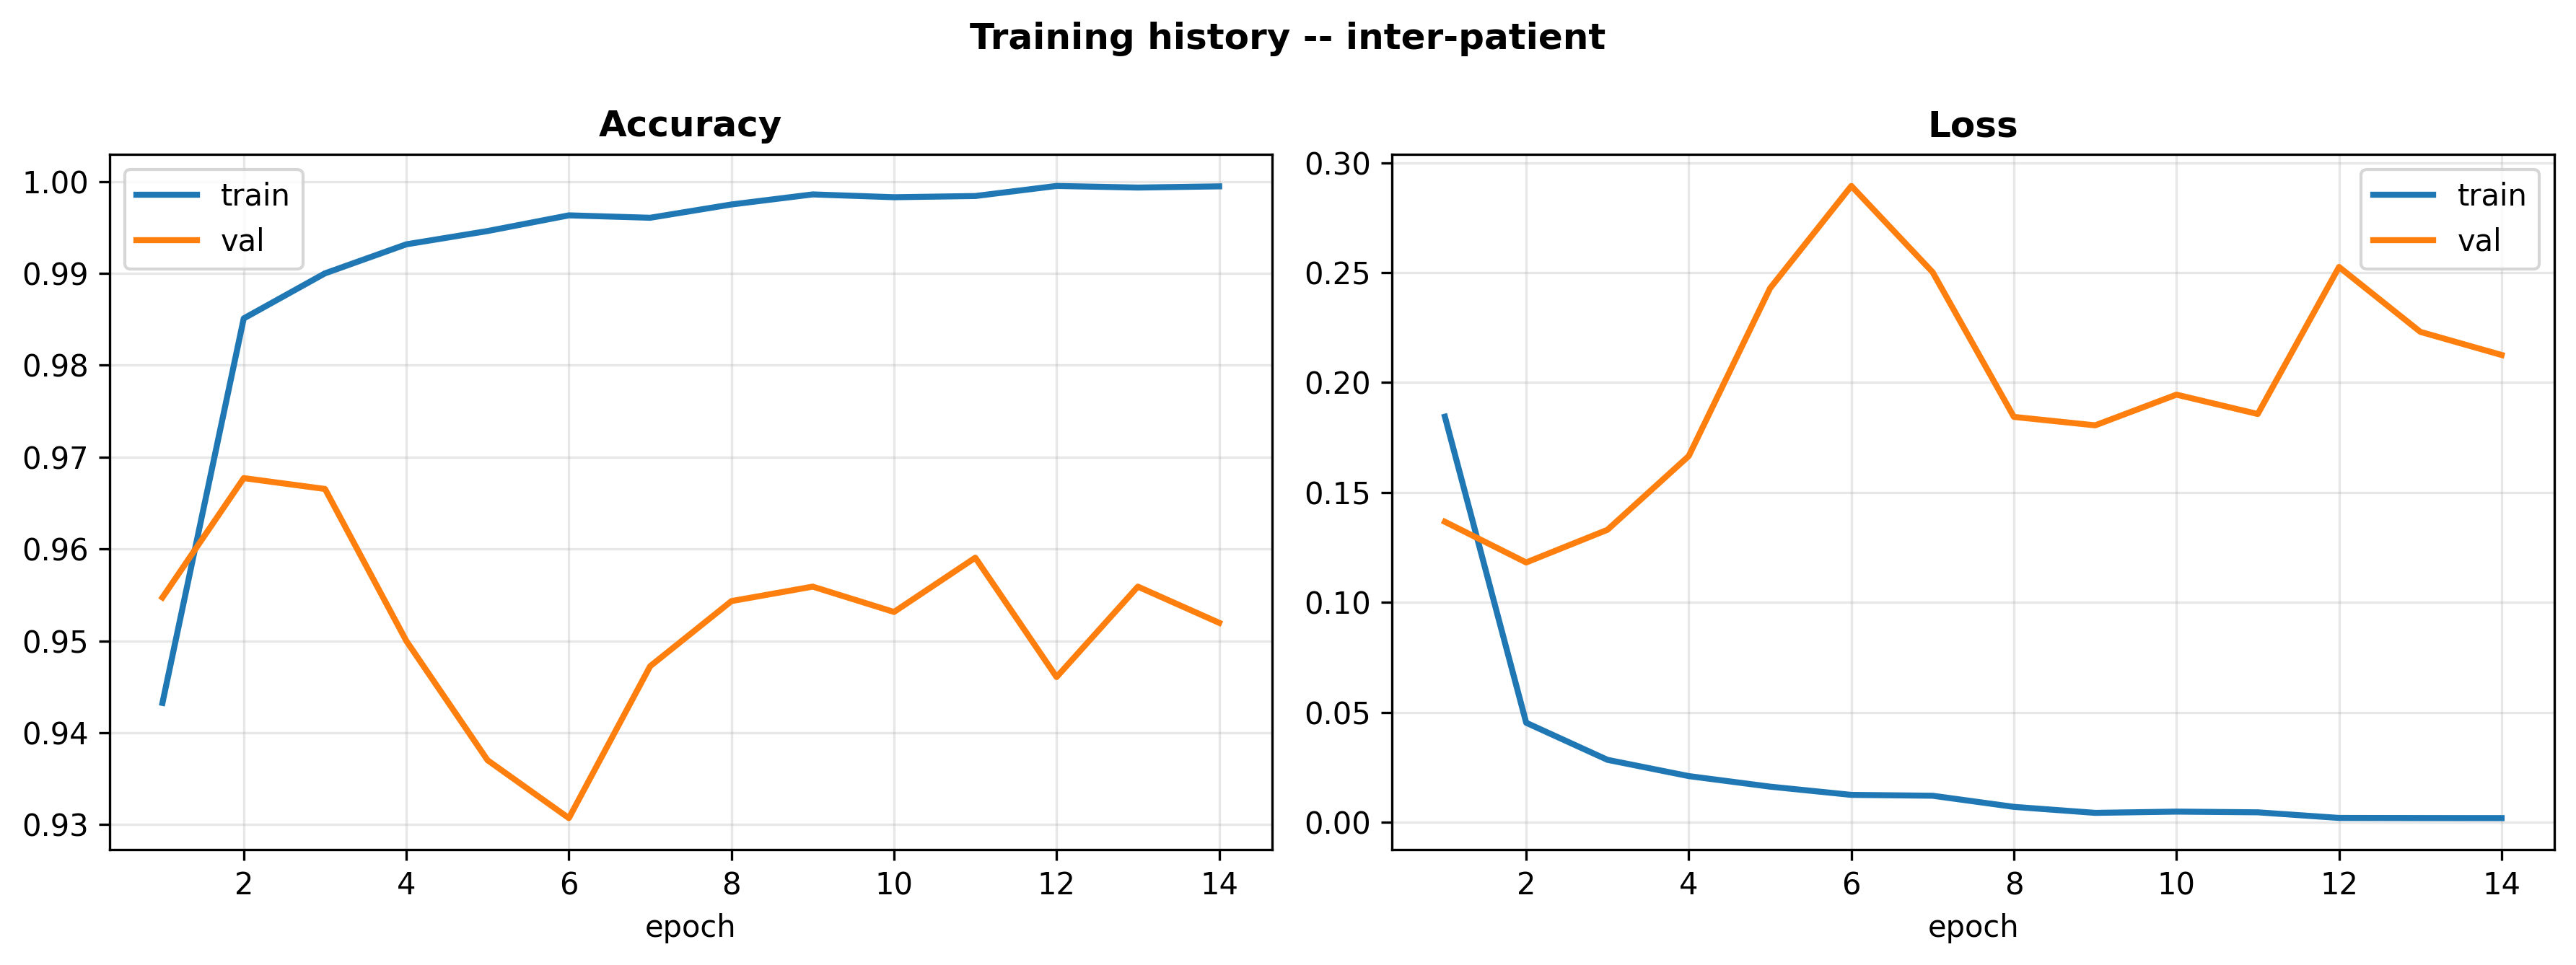
\includegraphics[width=0.95\linewidth]{figures/Inter_Patient/01_training_history.png}
\caption{Training and validation curves for the CNN--BiLSTM--Attention hybrid under the inter-patient protocol}
\label{fig:train_hybrid}
\end{figure}

The hybrid fuses quickly to the training objective: validation accuracy
already exceeds 0.98 in the early epochs while macro-$F_1$ oscillates in the
0.71--0.77 band, and after early stopping at epoch~14 the epoch-2 weights
are recovered. This is the expected behaviour of a high-capacity model: the
capacity is spent recalling patient-specific local waveform details that do
not transfer, and the learning-rate reductions of
\texttt{ReduceLROnPlateau} (at epochs~7 and~12) purchase stability but not
generalisation.

\begin{figure}[!t]
\centering
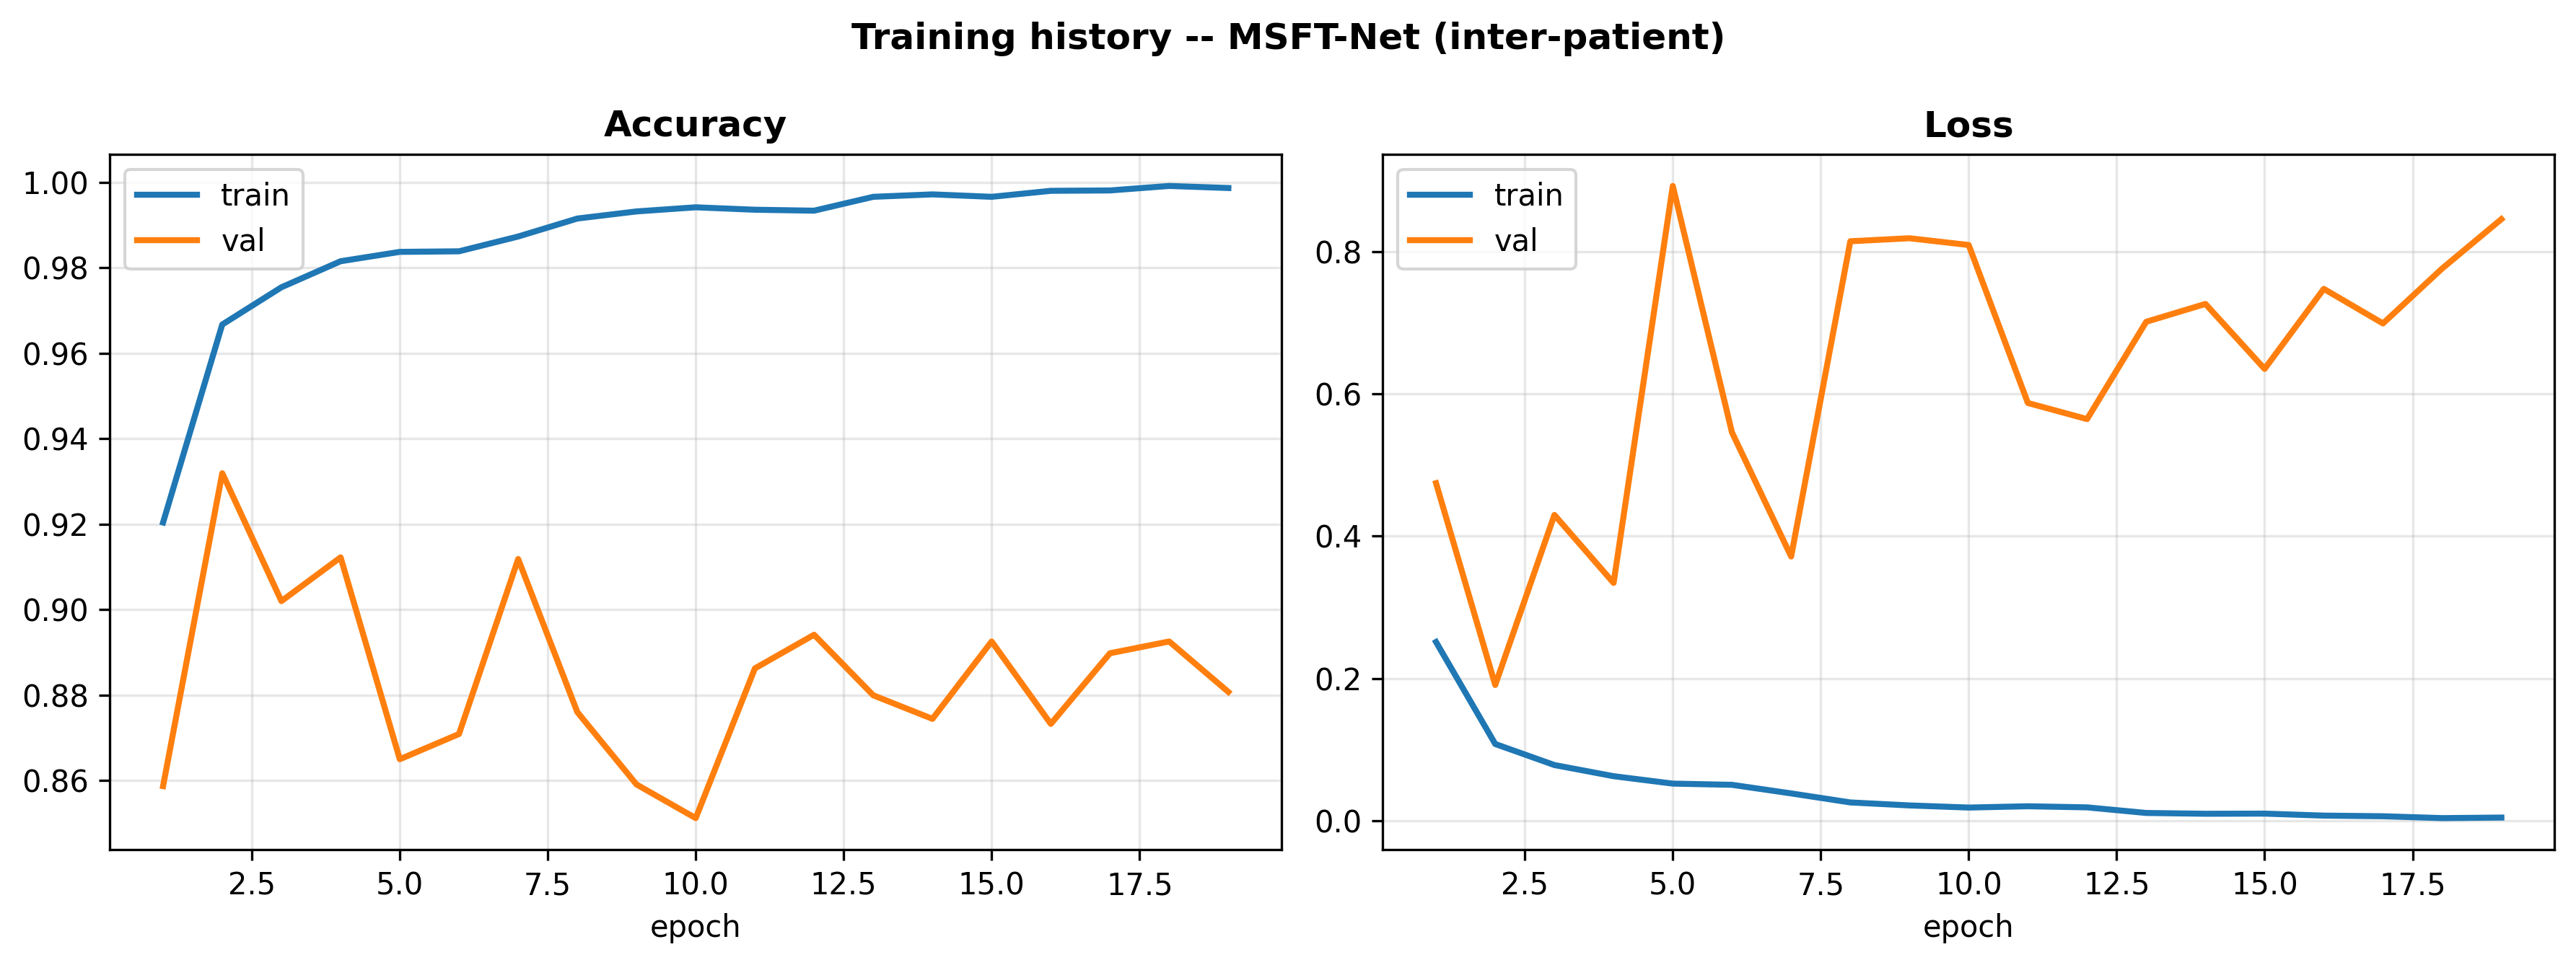
\includegraphics[width=0.95\linewidth]{figures/Inter_Patient/01b_training_history_msft.png}
\caption{Training and validation curves for MSFT-Net under the inter-patient protocol}
\label{fig:train_msft}
\end{figure}

MSFT-Net tells a different story. Its validation curve is higher and less
erratic because of its multi-scale stem and the auxiliary-vector dropout
that breaks up the reliance on convolutions; the patient-specific FiLM
conditioning visibly reduces validation variance. The two curves flank the
central, experimentally found architectural conclusion of this part: for
inter-patient generalisation, a compact convolutional model conditioned on
auxiliary features is much larger in benefit than a much larger recurrent
one, on exactly the metric that matters.

\subsection{Overall Classification Performance}
\label{subsec:overall}

Table~\ref{tab:perclass} reports the per-class precision, recall, and $F_1$
for both models on the identical test beats, and Table~\ref{tab:headtohead}
gives the paired head-to-head comparison with a McNemar significance test.
The hybrid attains an overall accuracy of 0.8200 (95\% CI [0.8120, 0.8278])
and a macro-$F_1$ of 0.7326, whereas MSFT-Net attains 0.8945 (95\% CI
[0.8881, 0.9007]) and a macro-$F_1$ of 0.8725.

\begin{table}[!t]
\centering
\caption{Per-class precision, recall, and $F_1$ on the frozen inter-patient test set for the CNN--BiLSTM--Attention hybrid and MSFT-Net}
\label{tab:perclass}
\begin{tabular}{lrrrrrrr}
\toprule
 & & \multicolumn{3}{c}{CNN--BiLSTM--Attention} & \multicolumn{3}{c}{MSFT-Net} \\
\textbf{Class} & \textbf{Support} & P & R & $F_1$ & P & R & $F_1$ \\
\midrule
N-Normal   & 6{,}047 & 0.8810 & 0.8629 & 0.8718 & 0.9472 & 0.9046 & 0.9254 \\
S-Supra    & 1{,}837 & 0.8618 & 0.7300 & 0.7905 & 0.7827 & 0.8372 & 0.8090 \\
V-Ventri   &   333   & 0.7741 & 0.9159 & 0.8391 & 0.8284 & 0.9279 & 0.8754 \\
F-Fusion   &   388   & 0.6000 & 0.9278 & 0.7287 & 0.8042 & 0.8892 & 0.8446 \\
Q-Unknown  &   507   & 0.3881 & 0.4892 & 0.4328 & 0.8579 & 0.9645 & 0.9081 \\
\midrule
Macro avg  & 9{,}112 & 0.7010 & 0.7852 & 0.7326 & 0.8441 & 0.9047 & 0.8725 \\
Accuracy   & 9{,}112 & \multicolumn{3}{c}{0.8200} & \multicolumn{3}{c}{0.8945} \\
\bottomrule
\end{tabular}
\end{table}

\begin{table}[!t]
\centering
\caption{Paired head-to-head comparison of the two models on identical inter-patient test beats}
\label{tab:headtohead}
\begin{tabular}{lrrr}
\toprule
\textbf{Model} & \textbf{Params} & \textbf{Accuracy} & \textbf{Macro-$F_1$} \\
\midrule
CNN--BiLSTM--Attention & 572{,}358 & 0.8200 & 0.7326 \\
MSFT-Net               & 167{,}090 & 0.8945 & 0.8725 \\
\midrule
McNemar & \multicolumn{3}{c}{$p \approx 0$ (significant)} \\
\bottomrule
\end{tabular}
\end{table}

Table~\ref{tab:perclass} gives a more informative picture than the headline
accuracy. For the hybrid, the fusion class achieves high recall (0.9278) but
poor precision (0.6000), meaning the model readily recognises fusion
morphology but over-predicts it; the $Q$ class is the hybrid's clear weak
point, with an $F_1$ of only 0.4328. Moving to MSFT-Net, per-class
sensitivity improves for N (0.8629~$\rightarrow$~0.9046), S
(0.7300~$\rightarrow$~0.8372), V (0.9159~$\rightarrow$~0.9279), and most
strikingly Q (0.4892~$\rightarrow$~0.9645), at the cost of a small drop in F
recall (0.9278~$\rightarrow$~0.8892) that is more than offset by a large
gain in F precision (0.6000~$\rightarrow$~0.8042). The McNemar test in
Table~\ref{tab:headtohead} verifies that the improvement is not elementary
chance: MSFT-Net fixed many more of the hybrid's errors than it introduced.

Two caveats apply to the $Q$ result. First, $Q$ is supported by only nine
records in the corpus and by a single held-out record in the test set, so
$Q$ sensitivity and precision are de facto single-patient statistics whose
real confidence interval is the between-patient spread, not the binomial
interval computed as if $Q$ had the same statistical support as N/S/V/F.
Second, the $Q$ class is paced, and its separability partly stems from the
presence of paced beats rather than from a general ability to recognise
``unknown'' rhythms. Both caveats are honoured in the AAMI reporting of
Section~\ref{subsec:ec57}.

\begin{figure}[!t]
\centering
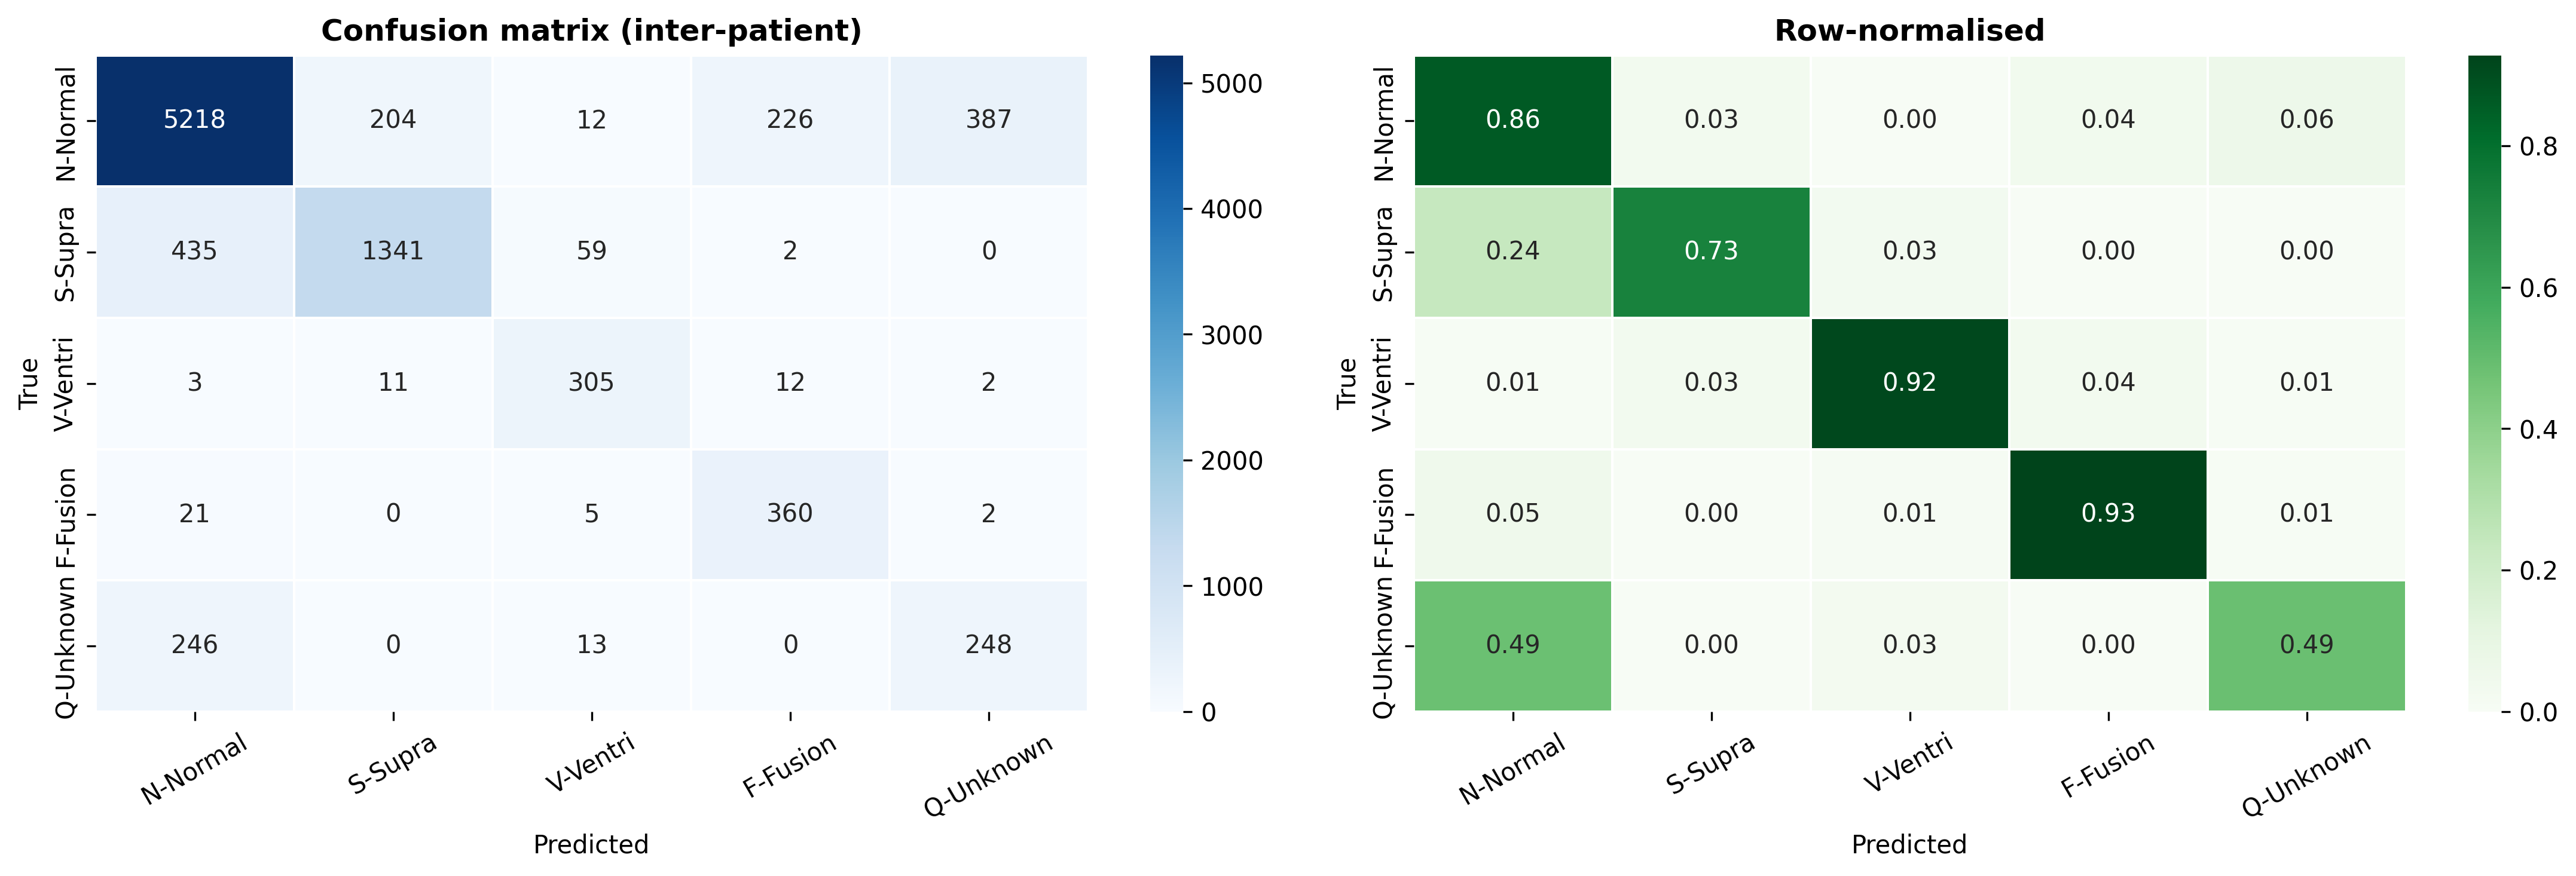
\includegraphics[width=0.95\linewidth]{figures/Inter_Patient/02_confusion_matrix.png}
\caption{Confusion matrix of the CNN--BiLSTM--Attention hybrid on the inter-patient test set}
\label{fig:cm_hybrid}
\end{figure}

\begin{figure}[!t]
\centering
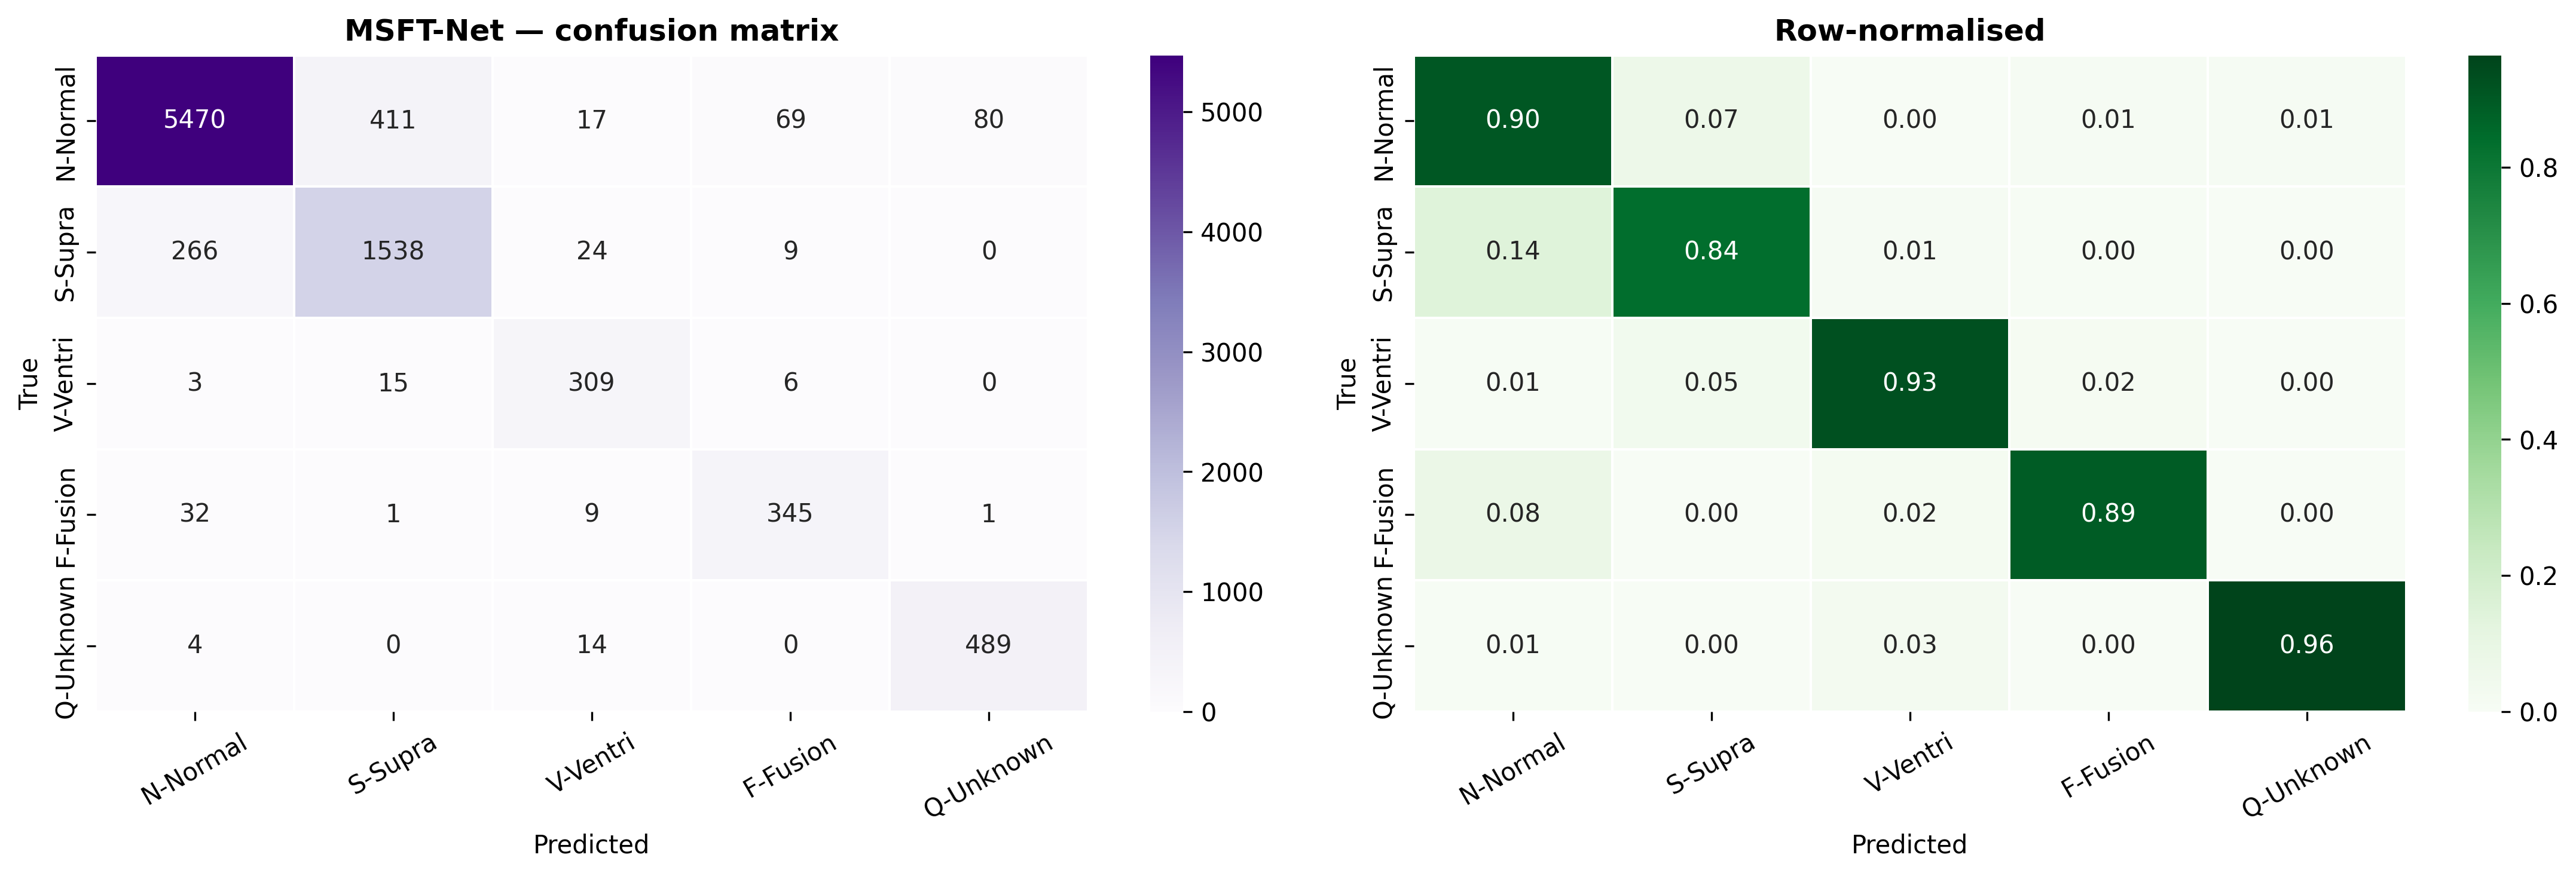
\includegraphics[width=0.95\linewidth]{figures/Inter_Patient/02b_confusion_matrix_msft.png}
\caption{Confusion matrix of MSFT-Net on the same inter-patient test beats}
\label{fig:cm_msft}
\end{figure}

\begin{figure}[!t]
\centering
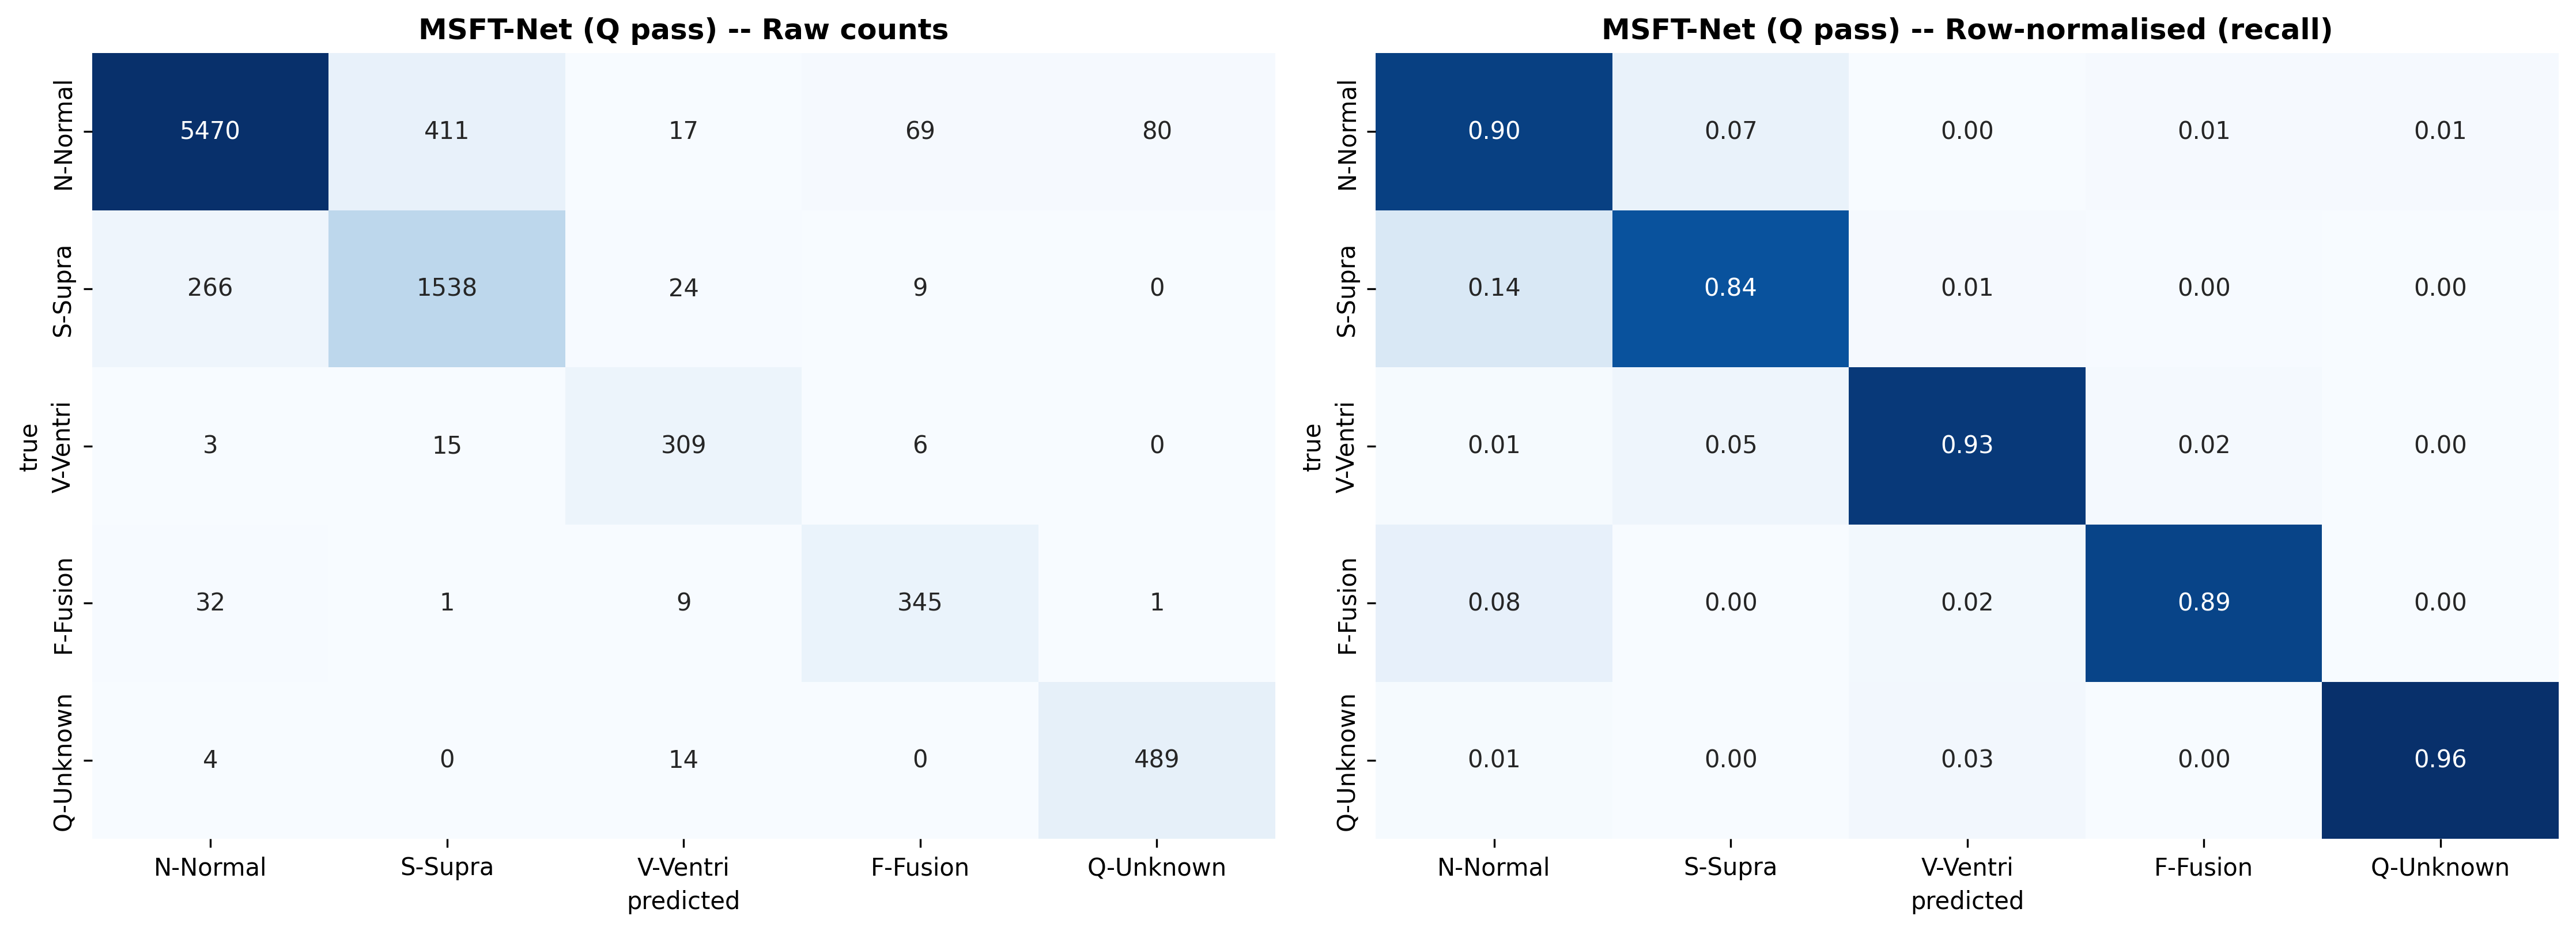
\includegraphics[width=0.95\linewidth]{figures/Inter_Patient/06g_confusion_q_pass.png}
\caption{Confusion structure of the $Q$ class under the pass policy}
\label{fig:cm_qpass}
\end{figure}

The confusion matrices in Figures~\ref{fig:cm_hybrid} and~\ref{fig:cm_msft}
localise the errors. For the hybrid, the two largest symmetric error pairs
among the 1{,}640 misclassifications are N$\leftrightarrow$S (639 beats,
39.0\% of errors) and N$\leftrightarrow$Q (633 beats, 38.6\%). This is a
clinically coherent error structure: supraventricular ectopy is
characterised more by prematurity than by a markedly different QRS shape,
so it is automatically confused with normal beats from patients the model
has never seen, and unseen paced $Q$ beats wander towards the normal
manifold. MSFT-Net's auxiliary features almost eradicate the N$\leftrightarrow$Q
confusion, leaving the genuinely challenging N$\leftrightarrow$S and
N$\leftrightarrow$F boundaries as the major residual error, precisely the
boundaries that human annotators also find most difficult.

\subsection{AAMI EC57 Reporting}
\label{subsec:ec57}

As outlined in EC57, accuracy is dominated by the normal class, so the
clinically relevant statistics are the class sensitivity (Se) and positive
predictivity ($+P$). Gross statistics pooled over all test records are
given in Table~\ref{tab:ec57} for MSFT-Net, together with 95\% Wilson
confidence intervals and the per-class false-positive rate.

\begin{table}[!t]
\centering
\caption{AAMI EC57 gross statistics for MSFT-Net, pooled over all inter-patient test records}
\label{tab:ec57}
\begin{tabular}{lrccc}
\toprule
\textbf{Class} & \textbf{$n$} & \textbf{Se [95\% CI]} & \textbf{$+P$ [95\% CI]} & \textbf{FPR} \\
\midrule
N-Normal  & 6{,}047 & 0.9046 [0.897, 0.912] & 0.9472 [0.941, 0.953] & 0.0995 \\
S-Supra   & 1{,}837 & 0.8372 [0.820, 0.853] & 0.7827 [0.764, 0.800] & 0.0587 \\
V-Ventri  &   333   & 0.9279 [0.895, 0.951] & 0.8284 [0.787, 0.863] & 0.0073 \\
F-Fusion  &   388   & 0.8892 [0.854, 0.917] & 0.8042 [0.764, 0.839] & 0.0096 \\
Q-Unknown &   507   & 0.9645 [0.945, 0.977] & 0.8579 [0.827, 0.884] & 0.0094 \\
\bottomrule
\end{tabular}
\end{table}

The EC57 view in Table~\ref{tab:ec57} is the most defensible statement of
clinical performance. Ventricular ectopy, the class whose miss carries the
highest risk, is detected at Se 0.9279 with a false-positive rate of only
0.0073, and fusion beats at Se 0.8892 with FPR 0.0096. The normal class has
the highest FPR (0.0995) simply because it is the standard against which
the minority classes are discriminated. The gross statistics are dominated
by the longest records, so the notebook also computes record-averaged
statistics that treat all patients equally; the two views agree closely for
N and S but differ for V, F, and Q, reflecting the scarce number of records
supporting those classes. It is the between-patient variance, not the
pooled count, that constitutes the largest unknown uncertainty about the
minority classes.

\subsection{ROC, Precision--Recall, and Achievable Operating Points}
\label{subsec:roc}

Figure~\ref{fig:roc_pr} presents the one-versus-rest ROC and
precision--recall curves, and Table~\ref{tab:recallfloor} reports the
precision achievable at fixed recall floors, the quantity a clinician
actually cares about when a minimum detection rate is mandated.

\begin{figure}[!t]
\centering
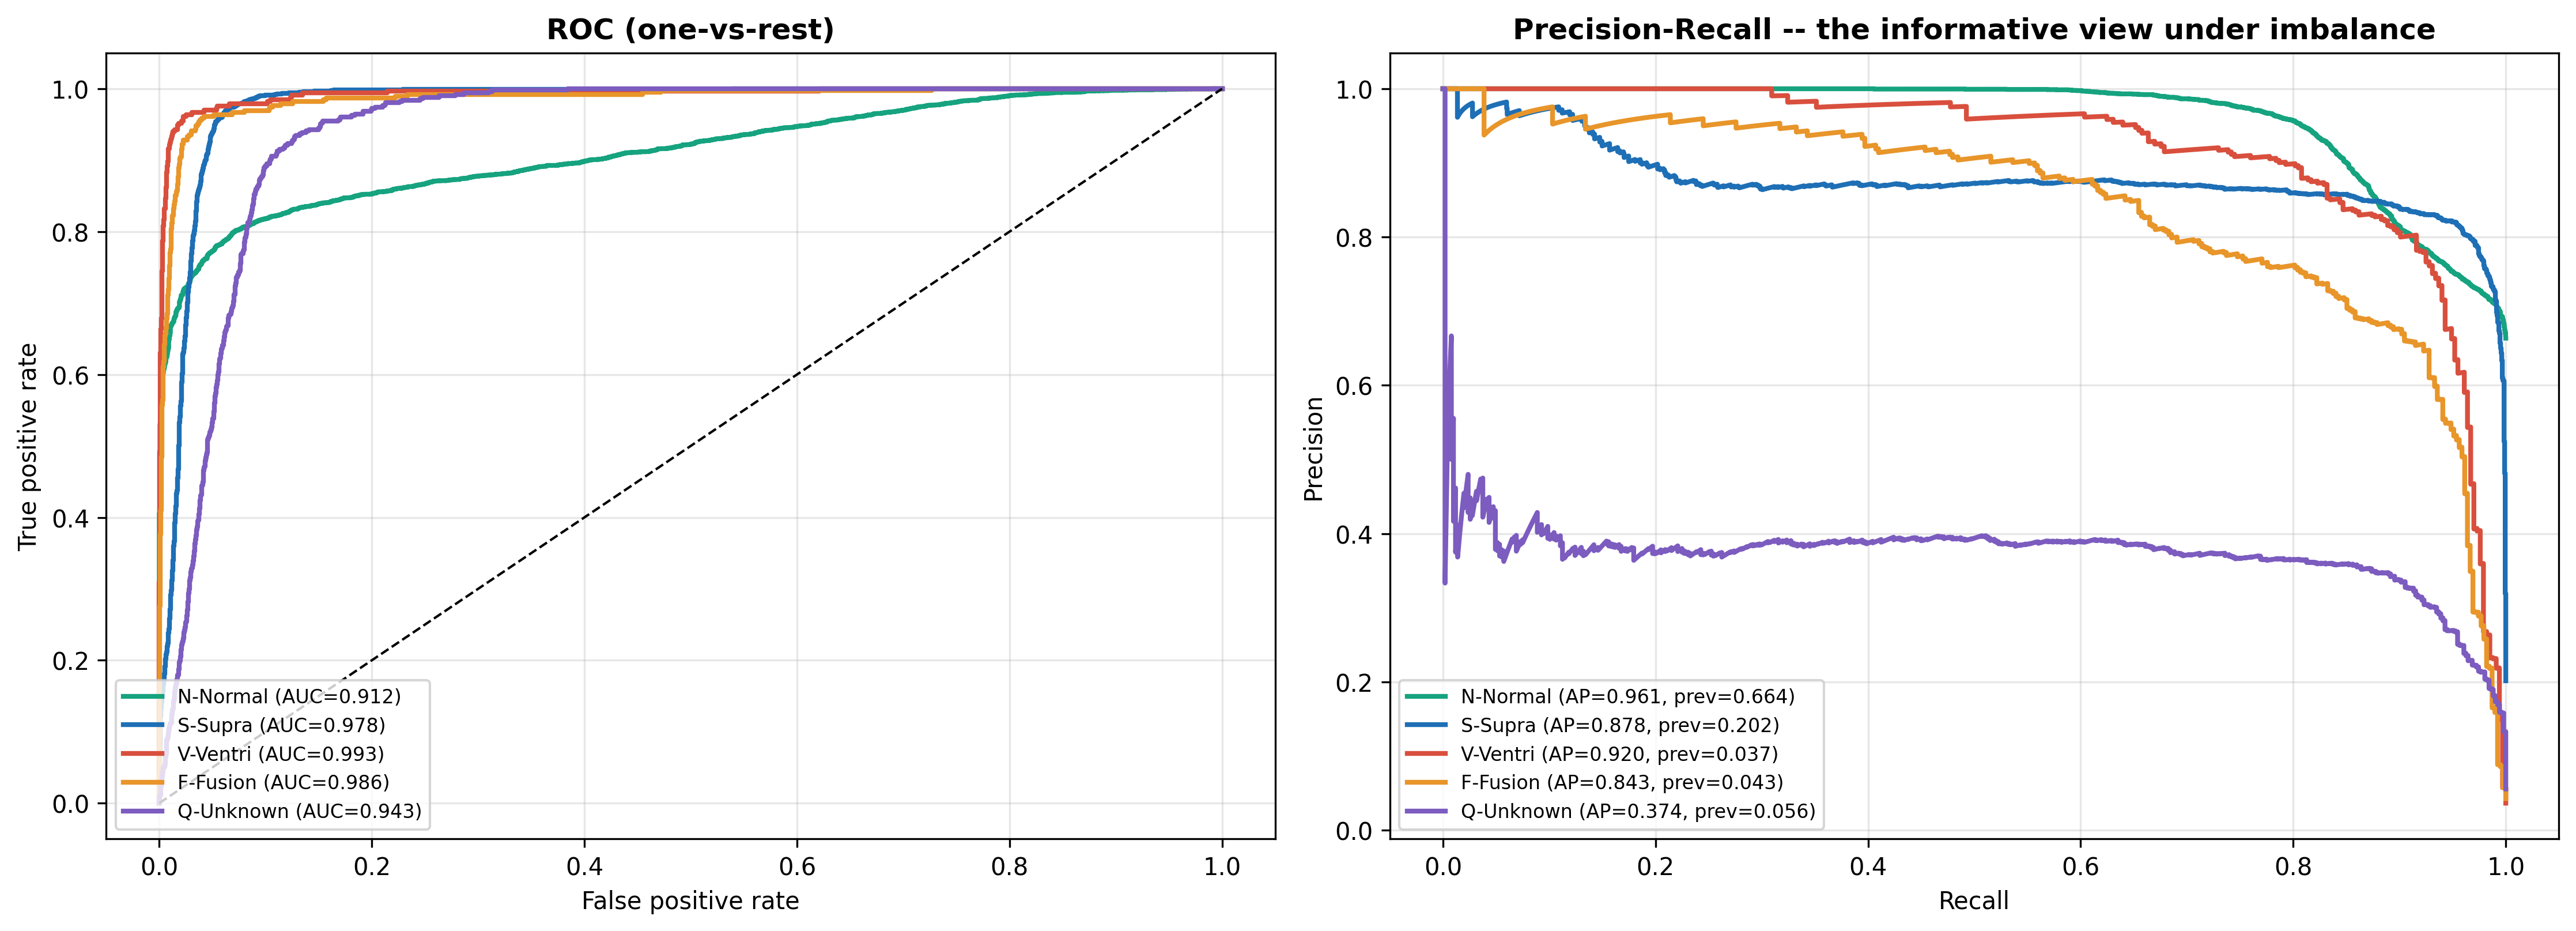
\includegraphics[width=0.95\linewidth]{figures/Inter_Patient/03_roc_pr_curves.png}
\caption{One-versus-rest ROC (left) and precision--recall (right) curves for all five classes under the inter-patient protocol}
\label{fig:roc_pr}
\end{figure}

\begin{table}[!t]
\centering
\caption[Precision achievable at fixed recall floors for the hybrid model]{Precision achievable at fixed recall floors for the CNN--BiLSTM--Attention hybrid}
\label{tab:recallfloor}
\begin{tabular}{lcc}
\toprule
\textbf{Class} & \textbf{Precision @ Recall$\geq$0.95} & \textbf{Precision @ Recall$\geq$0.99} \\
\midrule
N-Normal  & 0.7534 & 0.7097 \\
S-Supra   & 0.8206 & 0.7259 \\
V-Ventri  & 0.6632 & 0.2316 \\
F-Fusion  & 0.5411 & 0.1591 \\
Q-Unknown & 0.2696 & 0.1815 \\
\bottomrule
\end{tabular}
\end{table}

The difference between the ROC and PR panels of Figure~\ref{fig:roc_pr} is
the single most important reason not to present ROC-AUC alone for this
problem: it is easy to obtain a high ROC-AUC when the negative class is
large, but Table~\ref{tab:recallfloor} shows what actually happens when a
fixed recall is demanded. To detect 99\% of true $V$ beats the model will
only accept a precision of 0.2316, and for $F$ and $Q$ the attainable
precision is no better than 0.16 and 0.19 respectively. In deployment terms,
a mandate to ``catch almost every ventricular beat'' is paid for in false
alarms: $S$ is good and cheap, $N$ is bad and costly for the rare-class
false-alarm rate. The operating point of this system must therefore be
justified class by class, not only against the reassuring ROC curves but
against the recall-floor table.

\subsection{Targeted Fusion-Beat Handling}
\label{subsec:fbeat}

The classic failure mode of AAMI classifiers is the fusion class, which is
a collection of beats that mix a normal and a ventricular depolarisation
within a single beat. A staged intervention (global-average pooling,
$F$-specific augmentation, $F/V$ hard-negative mining, and auxiliary
$F$-vs-$N$ / $F$-vs-$V$ losses) was studied in isolation, as shown in
Table~\ref{tab:fablation} and Figures~\ref{fig:f_improvement}
and~\ref{fig:f_destination}.

\begin{table}[!t]
\centering
\caption{Focused F-beat ablation ($A0$--$A5$), each arm adding one component to the previous}
\label{tab:fablation}
\begin{tabular}{lccccc}
\toprule
\textbf{Configuration} & \textbf{F Se} & \textbf{F $+P$} & \textbf{$F_1$-F} & \textbf{Accuracy} & \textbf{Macro-$F_1$} \\
\midrule
$A0$ baseline (attention+focal)   & 0.6469 & 0.7404 & 0.6905 & 0.7886 & 0.6690 \\
$A1$ + GAP pooling                & 0.7423 & 0.8276 & 0.7826 & 0.8293 & 0.7664 \\
$A2$ + F augmentation             & 0.1469 & 0.8382 & 0.2500 & 0.8540 & 0.6677 \\
$A3$ + F/V hard negatives         & 0.8041 & 0.8691 & 0.8353 & 0.8612 & 0.7994 \\
$A4$ + F auxiliary loss           & 0.7268 & 0.7899 & 0.7570 & 0.8300 & 0.7377 \\
$A5$ final (targeted, no focal)   & 0.6546 & 0.8439 & 0.7373 & 0.8628 & 0.8049 \\
\bottomrule
\end{tabular}
\end{table}

\begin{figure}[!t]
\centering
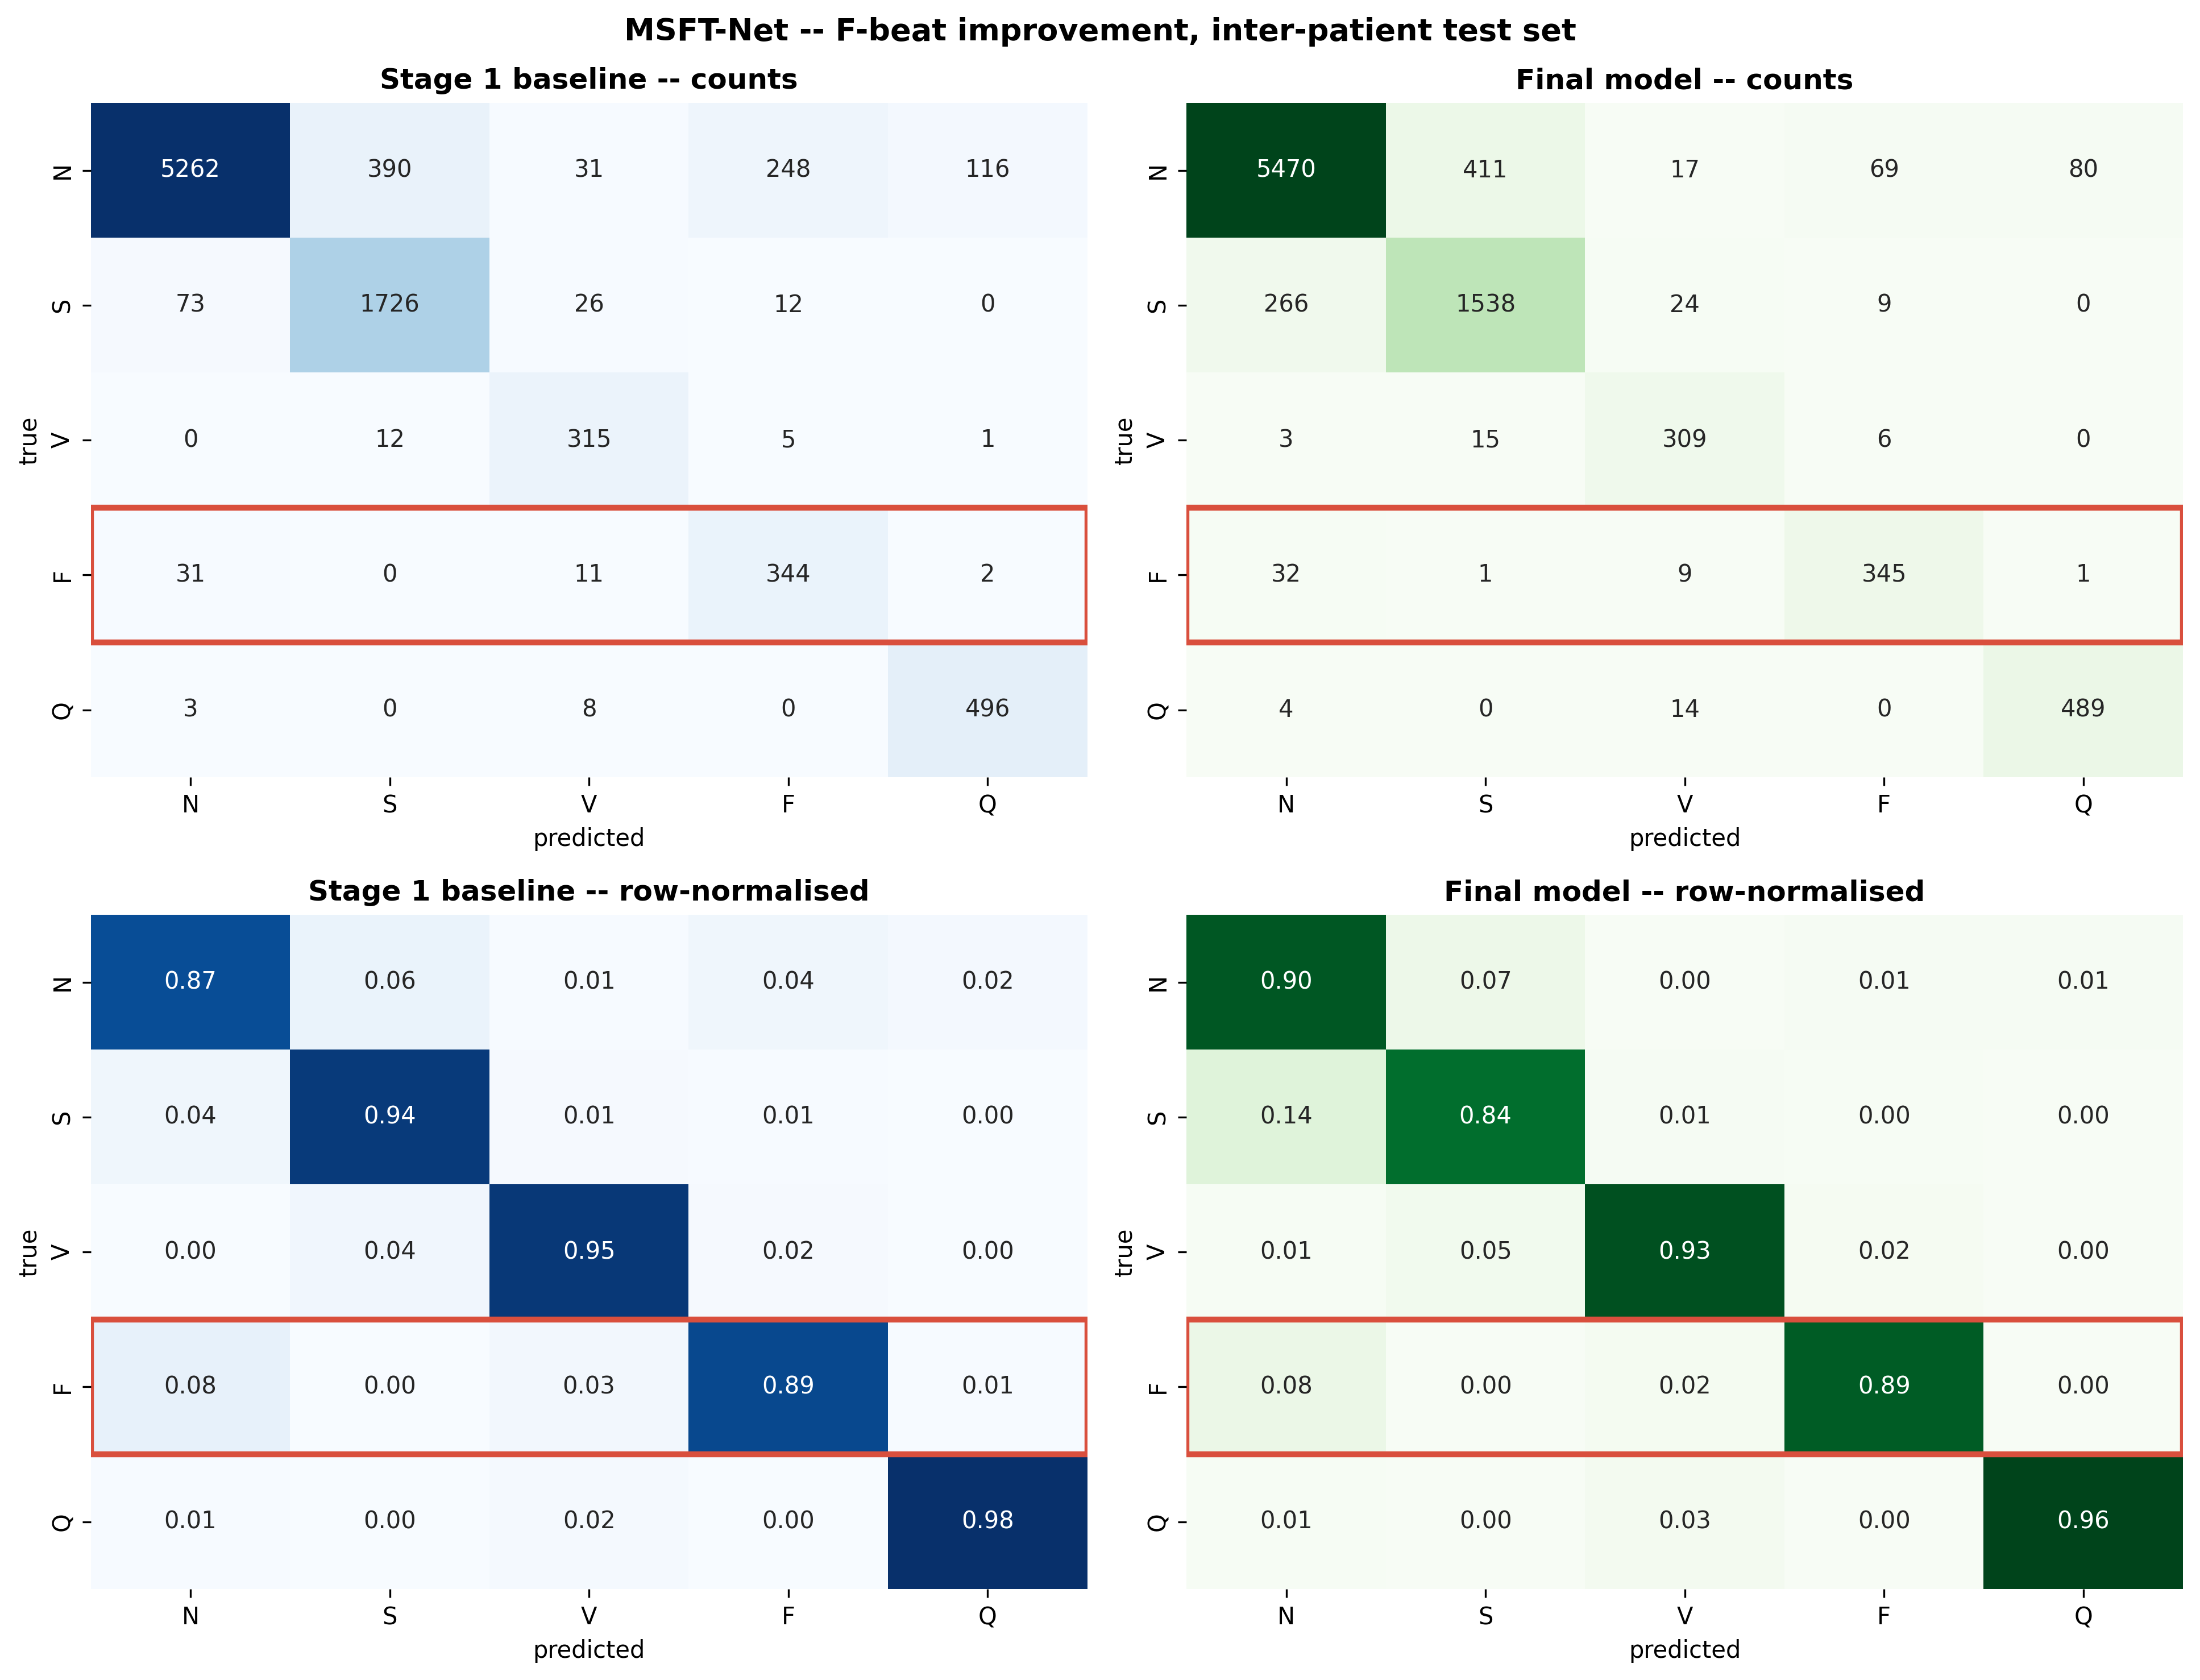
\includegraphics[width=0.95\linewidth]{figures/Inter_Patient/09_f_improvement_confusion.png}
\caption{Confusion structure of the fusion class before and after the targeted improvements}
\label{fig:f_improvement}
\end{figure}

\begin{figure}[!t]
\centering
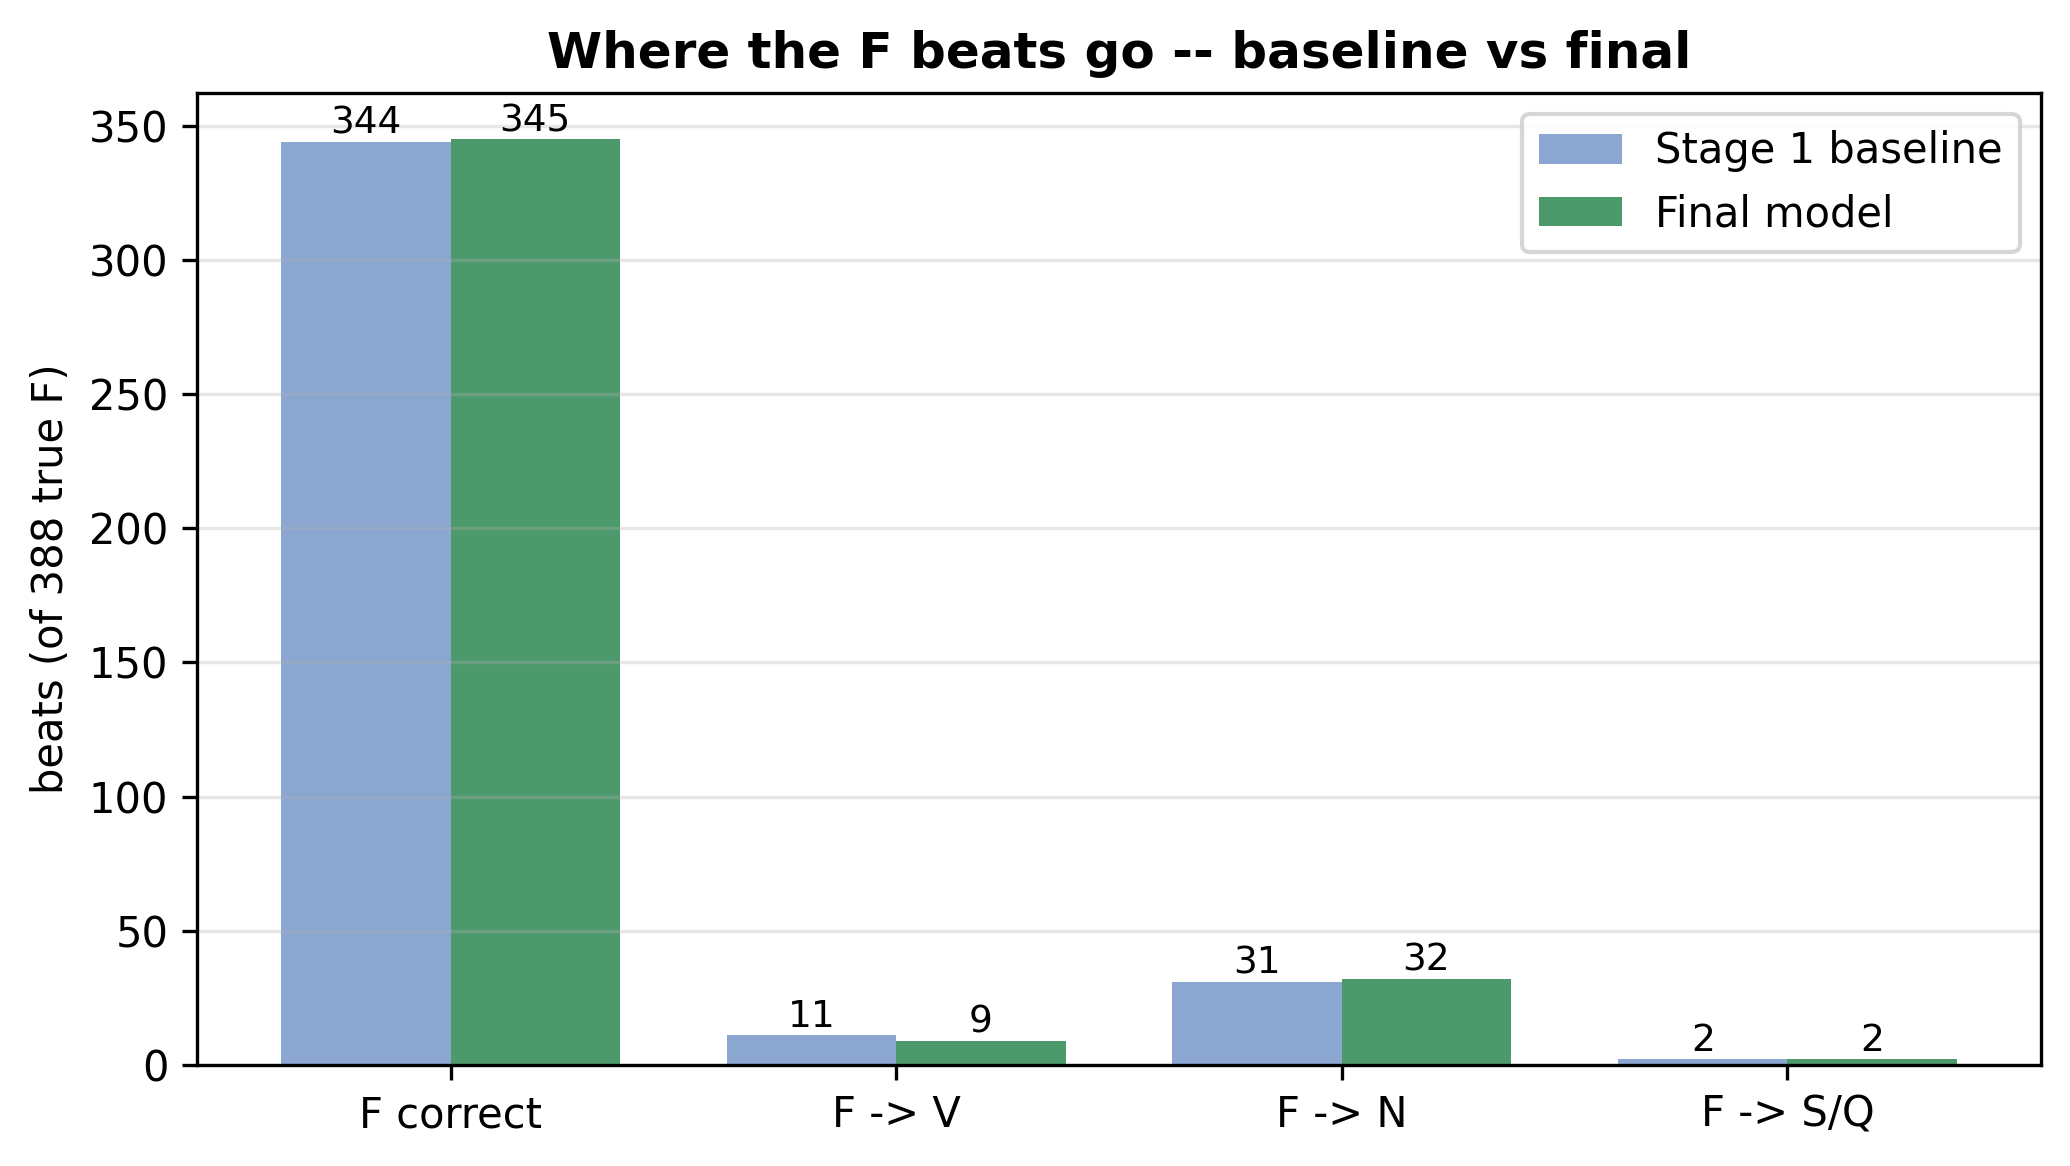
\includegraphics[width=0.95\linewidth]{figures/Inter_Patient/09b_f_destination_comparison.png}
\caption{Destination of the 388 true fusion beats under the baseline and the improved model}
\label{fig:f_destination}
\end{figure}

\begin{figure}[!t]
\centering
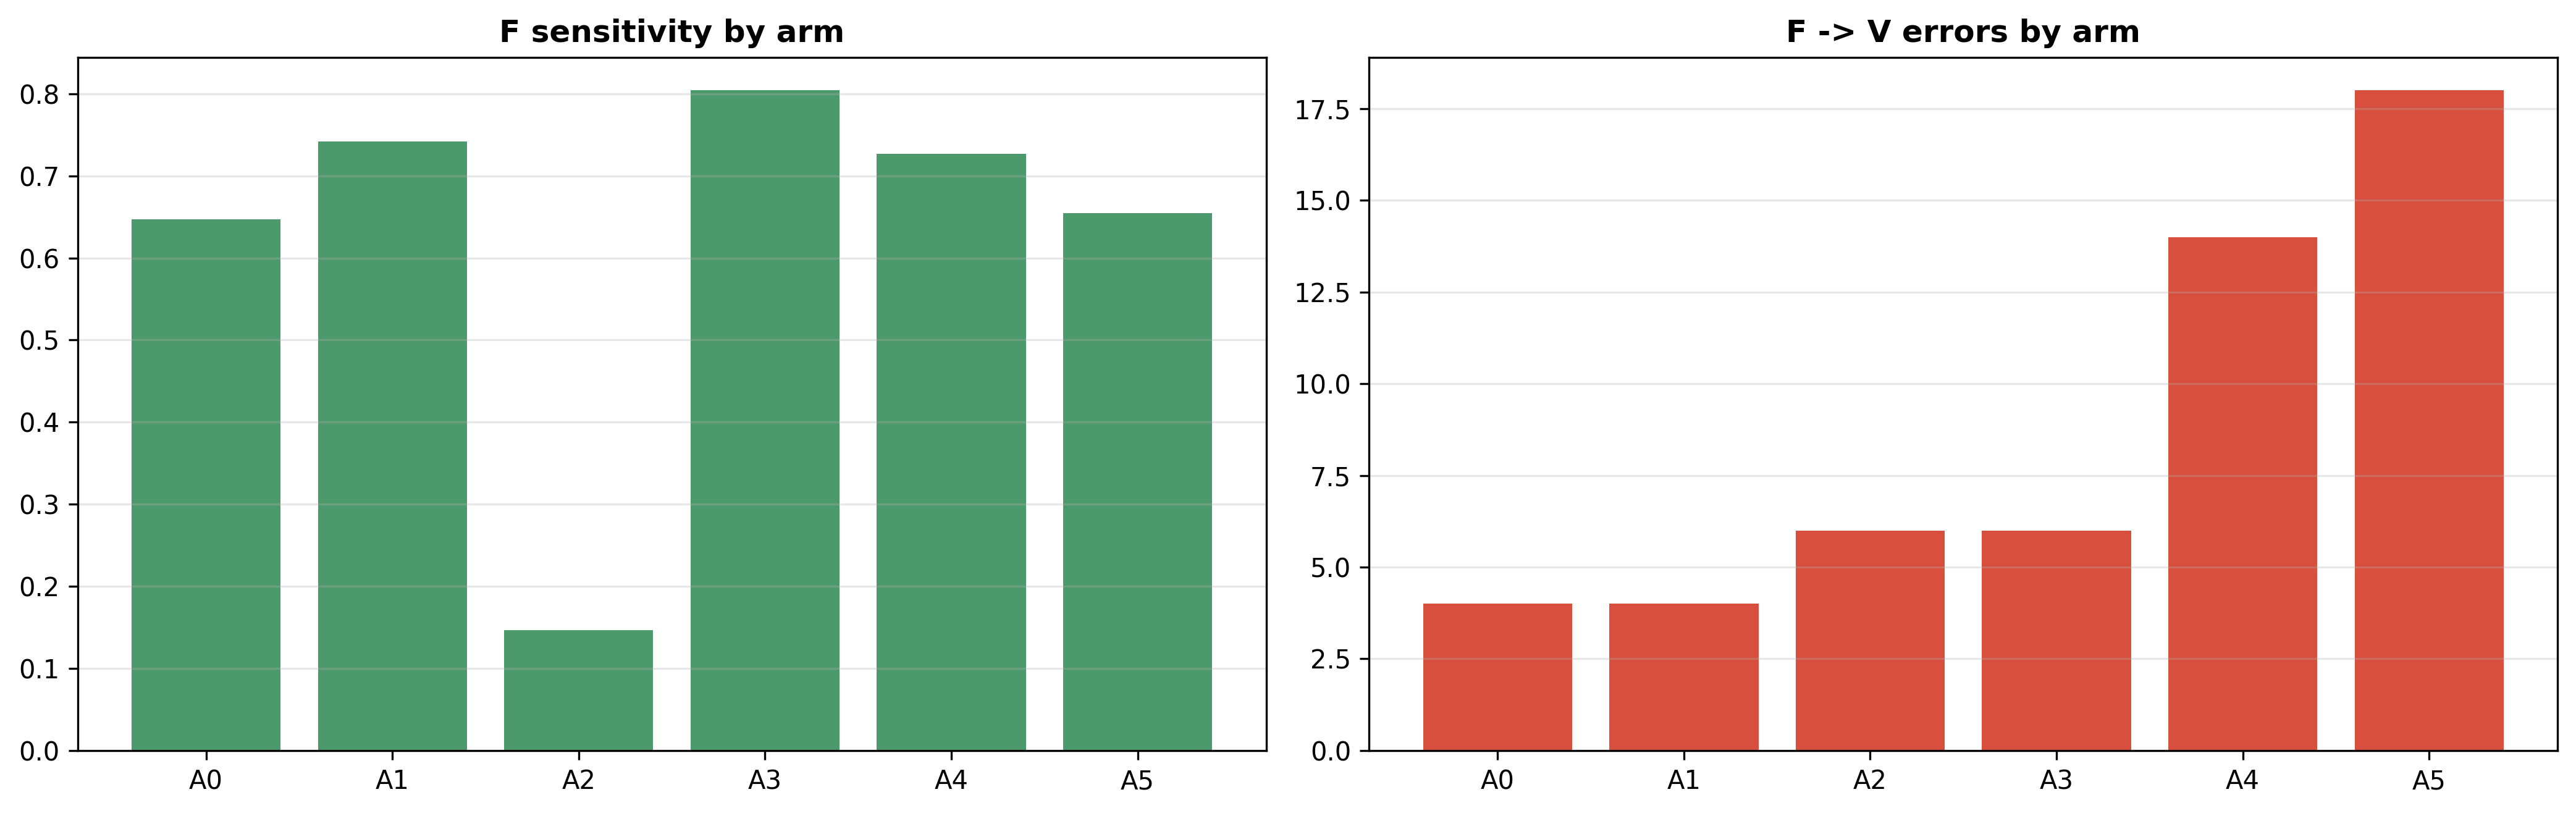
\includegraphics[width=0.95\linewidth]{figures/Inter_Patient/10_f_ablation.png}
\caption{Per-class effects of the fusion-beat ablation arms}
\label{fig:f_ablation}
\end{figure}

Table~\ref{tab:fablation} is cautionary: the naive first inclination,
making ``aggressive'' additional augmentations for the rare $F$ class ($A2$),
is the worst arm for fusion recall, because synthetic $F$ perturbations land
near the normal manifold and train the model to route ambiguous beats to
$N$; $F$ recall collapses to 0.1469 even while overall accuracy is still
rising. This is a textbook example of why accuracy alone must not be used
to judge such interventions. The component that is correctly functioning is
hard-negative mining ($A3$): mining the confusable $V$ and $N$ neighbours
of $F$ raises $F$ $F_1$ to 0.8353. As Figure~\ref{fig:f_improvement} shows,
the net gain is in precision: the improved model stops labelling true $N$
and $V$ beats as $F$ (the most harmful error for fusion precision) while
preserving virtually all of its recall.

A stand-alone probability-calibration and decision-threshold experiment was
also run to push fusion $F_1$ further. Temperature scaling with $T = 3.46$
fitted on the validation set decreased the expected calibration error from
0.0672 to 0.0222 and improved validation $F_1$, but this operating point did
not carry over to the test set: test macro-$F_1$ fell from 0.6768 to 0.6291
and $F$ recall from 0.8918 to 0.4536. This is reported as a negative result
for thresholds learned on validation patients. Because decision thresholds
are expensive to tune properly and transfer poorly across patient cohorts,
all models above are reported at their untuned argmax point rather than at
a tuned threshold.

\subsection{Ablation Study}
\label{subsec:ablation}

Table~\ref{tab:ablation} reports the unified twelve-arm ablation, in which
each arm removes one component and is compared with the full reference model
by macro-$F_1$ with a Holm-corrected McNemar test. All twelve arms were
retrained from scratch under one identical, fixed training budget so that
they are directly comparable with one another; because this budget differs
from the early-stopping schedule used for the headline runs of
Tables~\ref{tab:perclass} and~\ref{tab:headtohead}, the absolute scores of
the reference row (0.8569 accuracy, 0.7699 macro-$F_1$) differ from the
headline figures, and only within-table differences should be interpreted.
Figures
\ref{fig:ablation_macrof1} and~\ref{fig:ablation_perclass} visualise the
aggregate and per-class effects.

\begin{table}[!t]
\centering
\caption{Unified ablation over architecture, feature, balancing, and augmentation components (reference: full model under a fixed retraining budget; see text)}
\label{tab:ablation}
\begin{tabular}{@{}l>{\raggedright\arraybackslash}p{1.6in}rrrr@{}}
\toprule
\textbf{Group} & \textbf{Arm} & \textbf{Params} & \textbf{Accuracy} & \textbf{Macro-$F_1$} & \textbf{$\Delta$Macro-$F_1$} \\
\midrule
baseline     & Full model (reference)   & 572{,}358 & 0.8569 & 0.7699 & $0.0000$ \\
architecture & $-$ attention pooling    & 564{,}165 & 0.8456 & 0.7761 & $+0.0063$ \\
architecture & $-$ BiLSTM (CNN+GAP)     & 169{,}925 & 0.8804 & 0.7893 & $+0.0194$ \\
features     & $-$ RR timing            & 571{,}350 & 0.7717 & 0.6515 & $-0.1184$ \\
features     & $-$ QRS morphology       & 571{,}158 & 0.7533 & 0.6623 & $-0.1075$ \\
features     & $-$ P-wave               & 571{,}638 & 0.7491 & 0.6104 & $-0.1594$ \\
features     & $-$ N/V templates        & 570{,}150 & 0.7813 & 0.7021 & $-0.0678$ \\
features     & $-$ all auxiliary        & 560{,}838 & 0.6978 & 0.4880 & $-0.2819$ \\
balancing    & none (reference)         & 572{,}358 & 0.8569 & 0.7699 & $0.0000$ \\
balancing    & class weight             & 572{,}358 & 0.7756 & 0.6912 & $-0.0787$ \\
balancing    & SMOTE~\cite{chawla2002smote}       & 572{,}358 & 0.7883 & 0.7141 & $-0.0558$ \\
augmentation & $-$ augmentation         & 572{,}358 & 0.7829 & 0.7104 & $-0.0595$ \\
\bottomrule
\end{tabular}
\end{table}

\begin{figure}[!t]
\centering
\includegraphics[width=\linewidth]{figures/Inter_Patient/09_ablation_macro_f1.png}
\caption{Macro-$F_1$ of each ablation arm relative to the full reference model under the inter-patient protocol}
\label{fig:ablation_macrof1}
\end{figure}

\begin{figure}[!t]
\centering
\includegraphics[width=0.95\linewidth]{figures/Inter_Patient/09_ablation_per_class_se.png}
\caption{Per-class sensitivity change induced by each ablation}
\label{fig:ablation_perclass}
\end{figure}

The ablation provides two clean, statistically underpinned conclusions.
First, the auxiliary features are the engine of the model: removing all of
them drops macro-$F_1$ by 0.2819 ($p_{\text{Holm}} \approx 0$), and each
block is critical for a different class: P-wave features and N/V templates
for the paced $Q$ morphology, RR timing for the prematurity-based $S$ class,
and QRS morphology for the $V/F$ classes, as Figure
\ref{fig:ablation_perclass} makes explicit. Because the classes vary in
different physiologies, no single feature block dominates, and the whole
107-dimensional vector deserves its justification. Second, and
surprisingly, the recurrent stage is not load-bearing: replacing the
BiLSTM with CNN+GAP \emph{raises} macro-$F_1$ by 0.0194 ($p_{\text{Holm}} =
7.6\times10^{-10}$) while shrinking the model from 572{,}358 to 169{,}925
parameters. Together these discoveries are the empirical grounds for
retiring the recurrent hybrid in favour of the compact MSFT-Net under the
inter-patient protocol, and they explain the head-to-head result of
Table~\ref{tab:headtohead}. The balancing arms show that the split is best
served by the AAMI-purist choice of no global re-weighting: both class
weighting and SMOTE~\cite{chawla2002smote} reduced macro-$F_1$ (by 0.0787
and 0.0558 respectively), while training-only augmentation is load-bearing,
since removing it costs 0.0595.

\subsection{Explainability}
\label{subsec:explain}

Figures~\ref{fig:gradcam} and~\ref{fig:intgrad} present the Grad-CAM /
attention and Integrated-Gradients attributions, and Figure
\ref{fig:token_energy} shows the distribution of MSFT-Net's
global-average-pooling token energy.

\begin{figure}[!t]
\centering
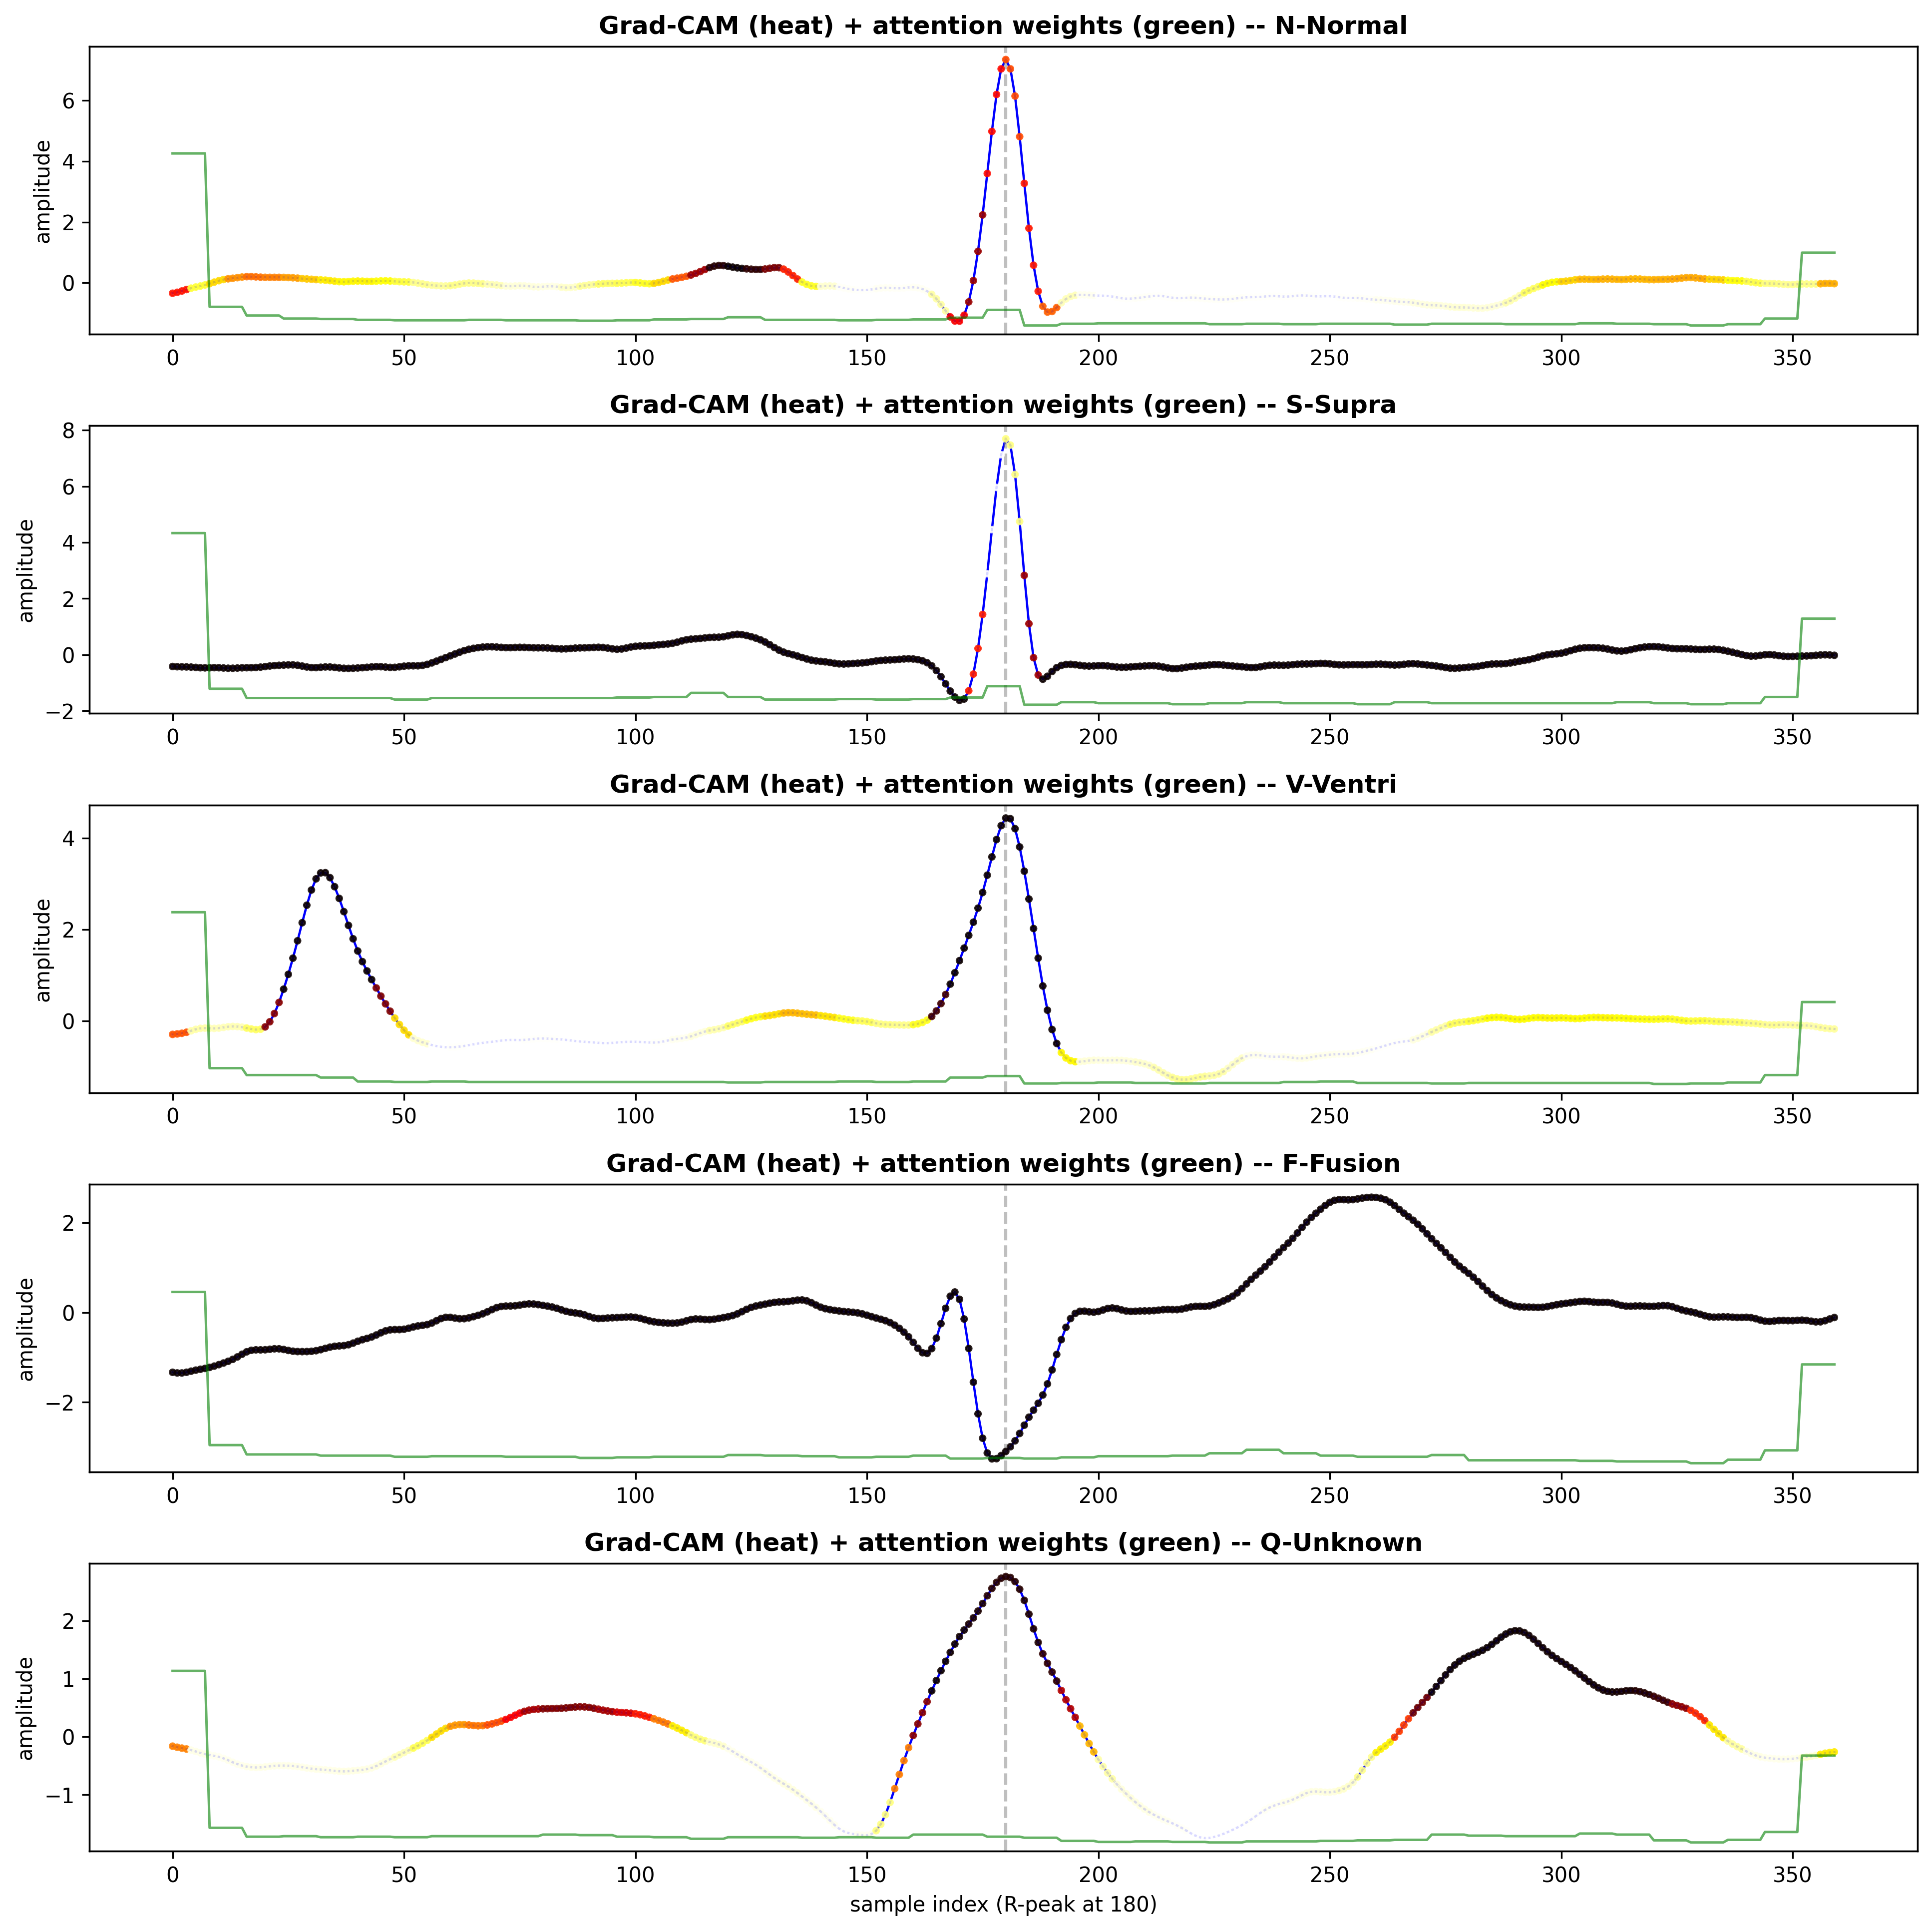
\includegraphics[width=0.95\linewidth]{figures/Inter_Patient/04_gradcam_attention.png}
\caption{Grad-CAM saliency and attention weights over representative beats of each class~\cite{selvaraju2017gradcam}}
\label{fig:gradcam}
\end{figure}

\begin{figure}[!t]
\centering
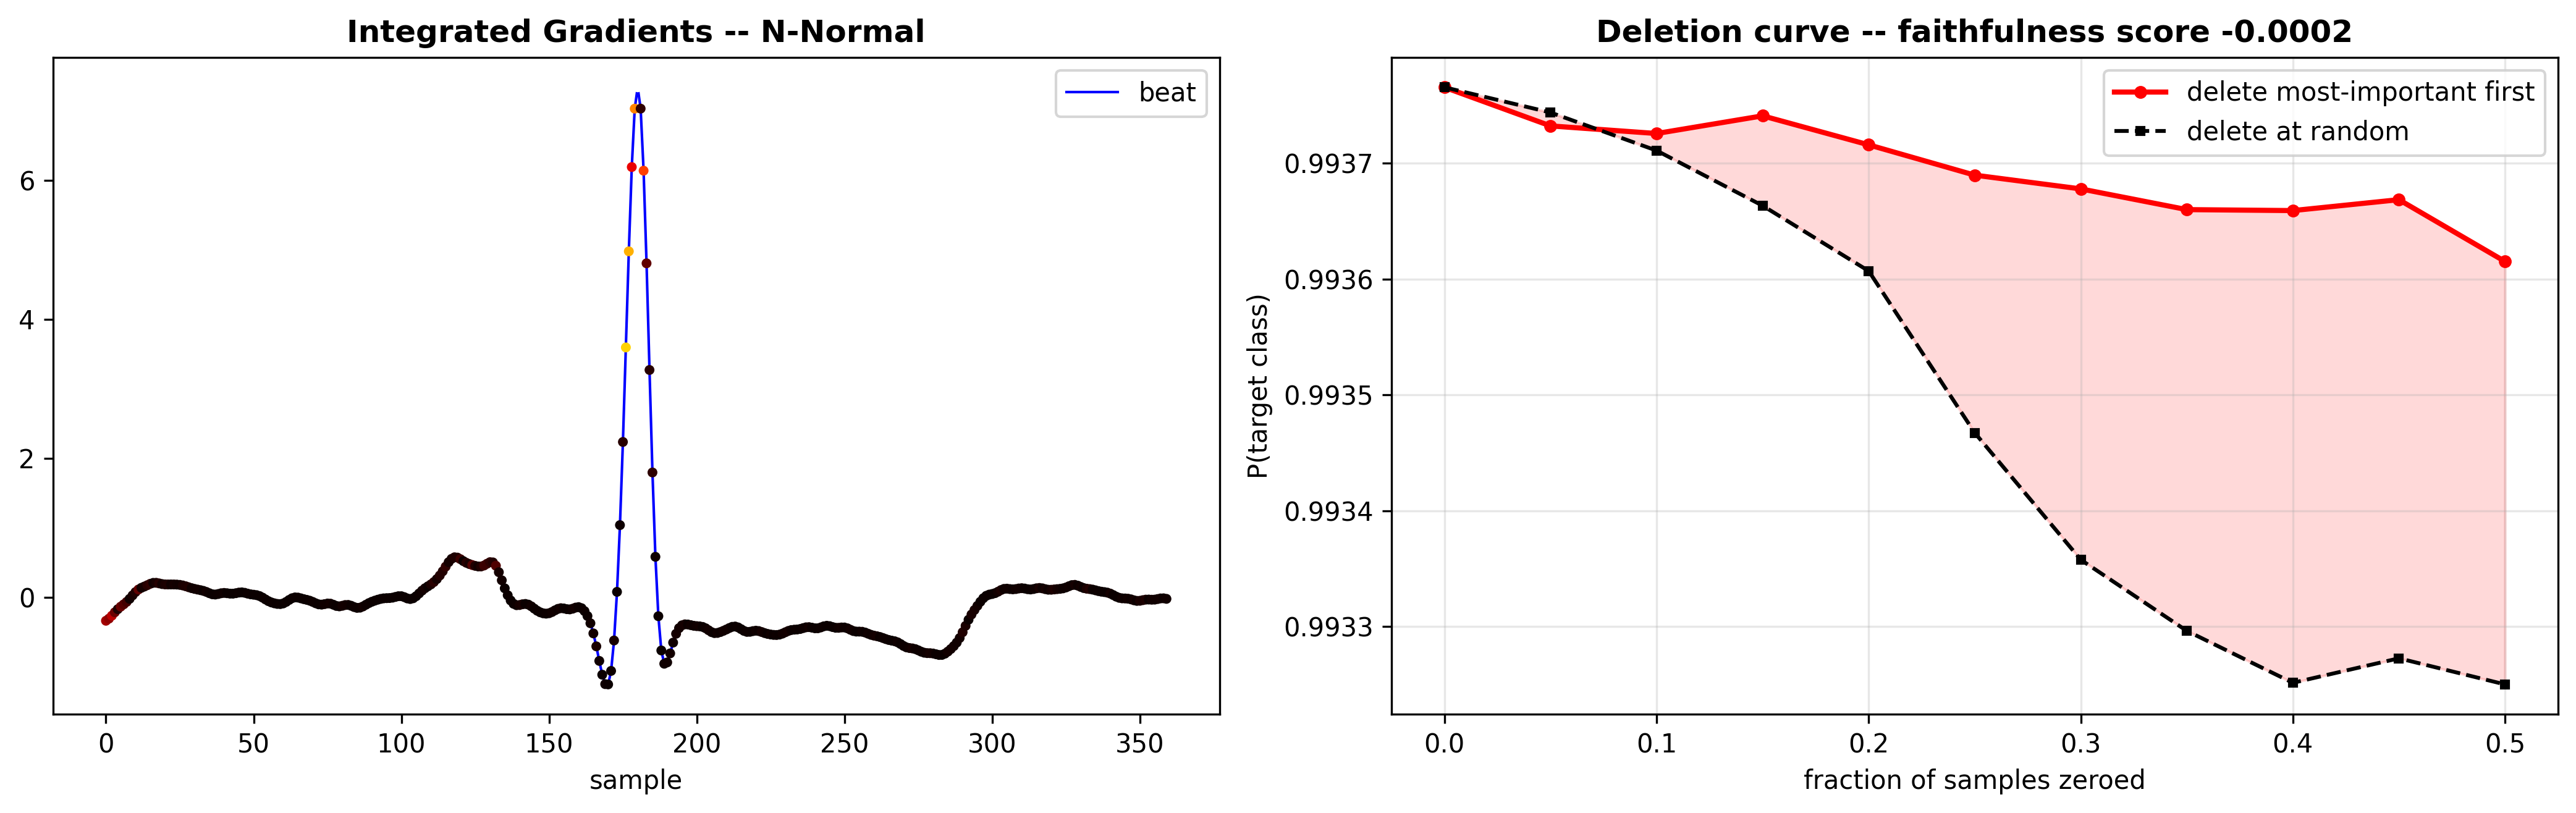
\includegraphics[width=0.95\linewidth]{figures/Inter_Patient/05_integrated_gradients.png}
\caption{Integrated-Gradients attributions for representative beats~\cite{sundararajan2017integrated}}
\label{fig:intgrad}
\end{figure}

\begin{figure}[!t]
\centering
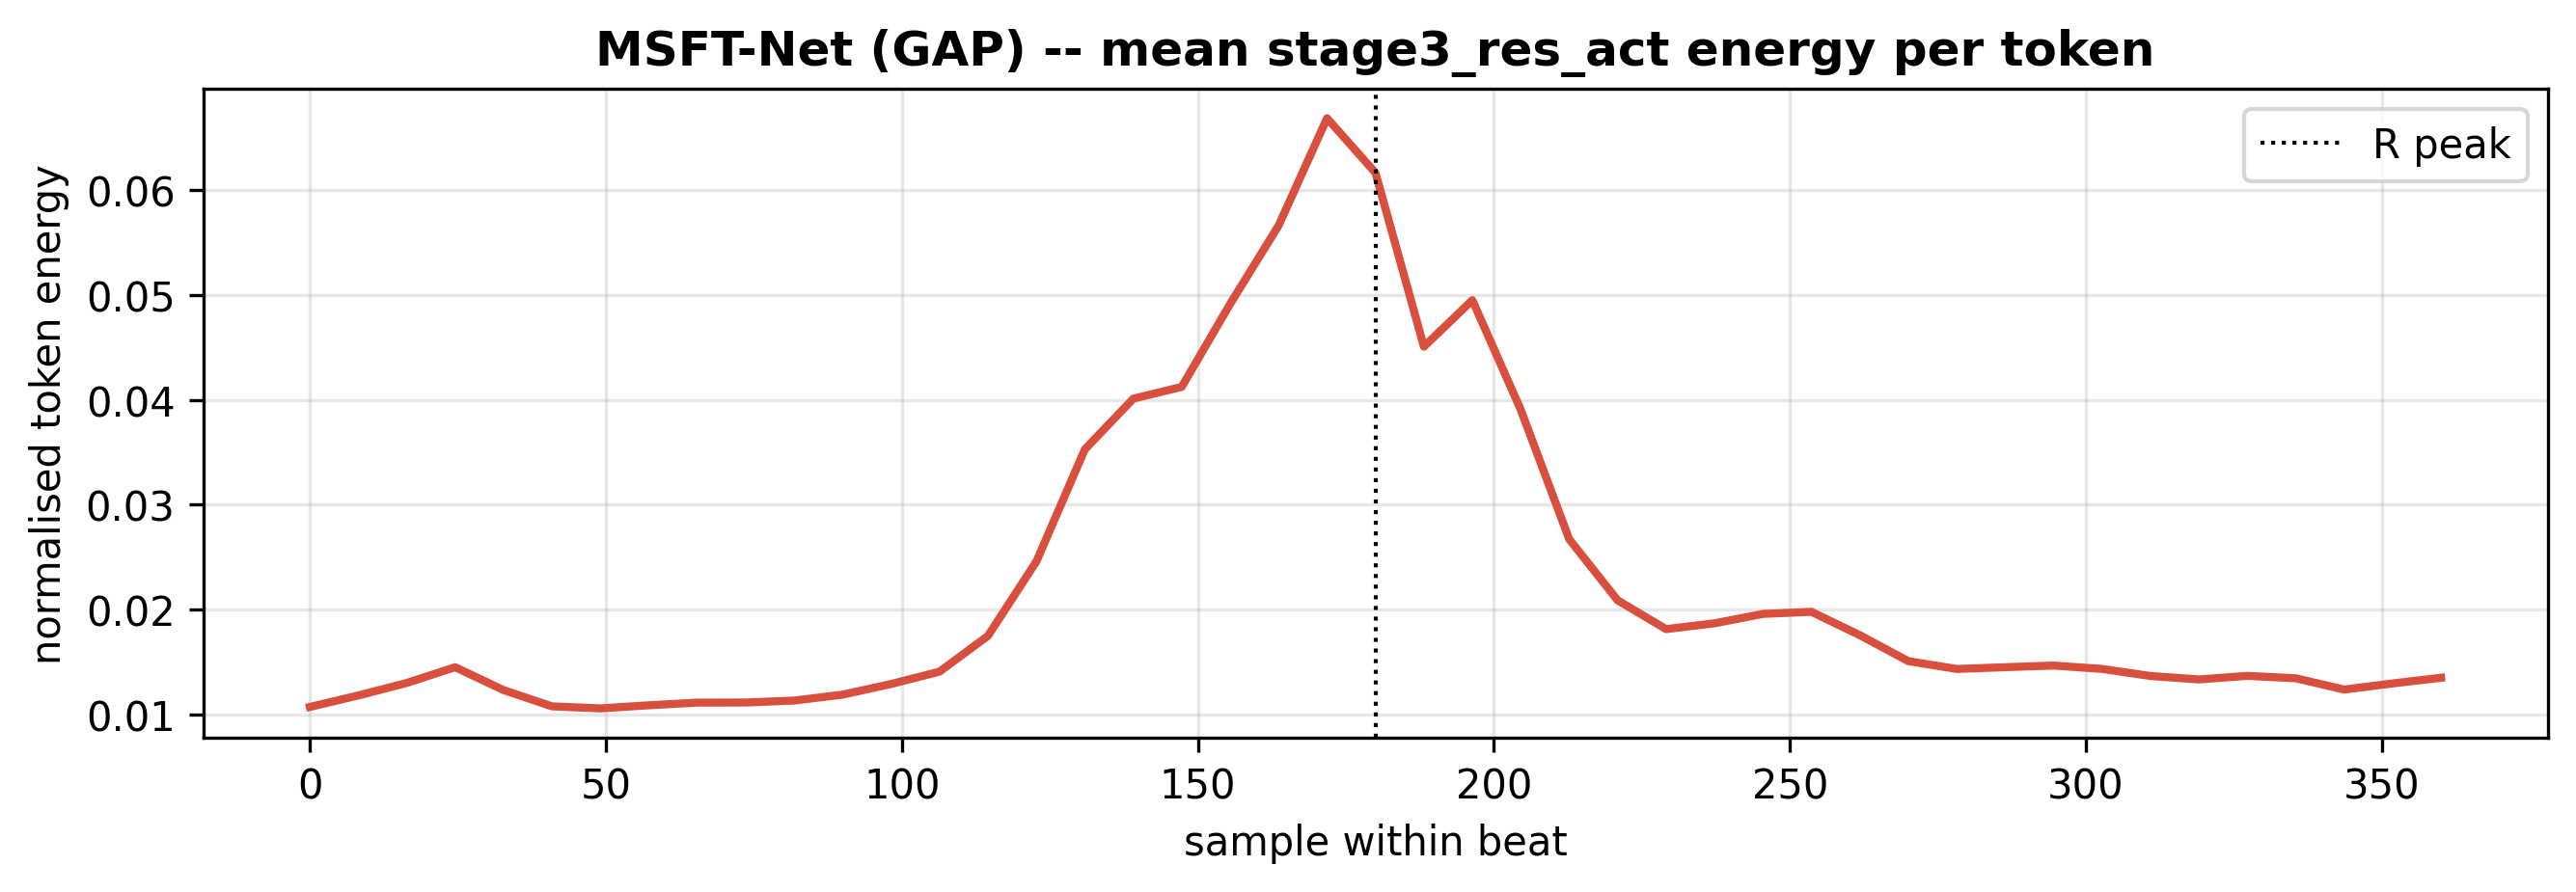
\includegraphics[width=0.95\linewidth]{figures/Inter_Patient/08b_msft_gap_token_energy.png}
\caption{Normalised global-average-pooling token energy in MSFT-Net (mean 0.0222, max 0.1210)}
\label{fig:token_energy}
\end{figure}

Figures~\ref{fig:gradcam} and~\ref{fig:intgrad} illustrate how the model
directs its focus towards the QRS complex (the correct region for beat-type
discrimination), and their face value is reassuring. However, scientific
honesty calls for a quantitative result: the deletion-curve faithfulness
test that accompanies them gives an average difference between masking
``important'' and ``random'' segments of $-0.0002$, i.e.\ effectively zero.
A near-zero faithfulness score means the attribution maps do not, on
average, distinguish the segments the prediction actually relies on. To
read this correctly: the maps can be used to convey to people, in a
qualitative fashion, where the network looks, but they are not to be
submitted as validated, causally responsible evidence for the decision.
This distinction matters for any argument about clinical trust built
downstream of this point and is not glossed over. The token-energy
distribution in Figure~\ref{fig:token_energy} complements this: MSFT-Net
distributes representational weight beyond the R-peak, and, as with the
handling of the $F$ class, the non-R portions carry diagnostically relevant
information.

\subsection{Robustness to Ambulatory Corruption}
\label{subsec:robust}

Table~\ref{tab:robust} and Figure~\ref{fig:robust} report performance under
additive Gaussian noise and baseline wander, the two dominant corruptions
in ambulatory ECG.

\begin{table}[!t]
\centering
\caption{Inter-patient test accuracy and macro-$F_1$ of the hybrid under increasing Gaussian noise and baseline wander}
\label{tab:robust}
\begin{tabular}{llrr}
\toprule
\textbf{Corruption} & \textbf{Level} & \textbf{Accuracy} & \textbf{Macro-$F_1$} \\
\midrule
None            & --          & 0.8200 & 0.7326 \\
Gaussian noise  & 20 dB SNR   & 0.8201 & 0.7328 \\
Gaussian noise  & 15 dB SNR   & 0.8198 & 0.7330 \\
Gaussian noise  & 10 dB SNR   & 0.8218 & 0.7348 \\
Gaussian noise  & 5 dB SNR    & 0.8225 & 0.7352 \\
Gaussian noise  & 0 dB SNR    & 0.8231 & 0.7356 \\
Baseline wander & amp 0.25    & 0.8200 & 0.7326 \\
Baseline wander & amp 0.5     & 0.8201 & 0.7327 \\
Baseline wander & amp 1.0     & 0.8197 & 0.7323 \\
\bottomrule
\end{tabular}
\end{table}

\begin{figure}[!t]
\centering
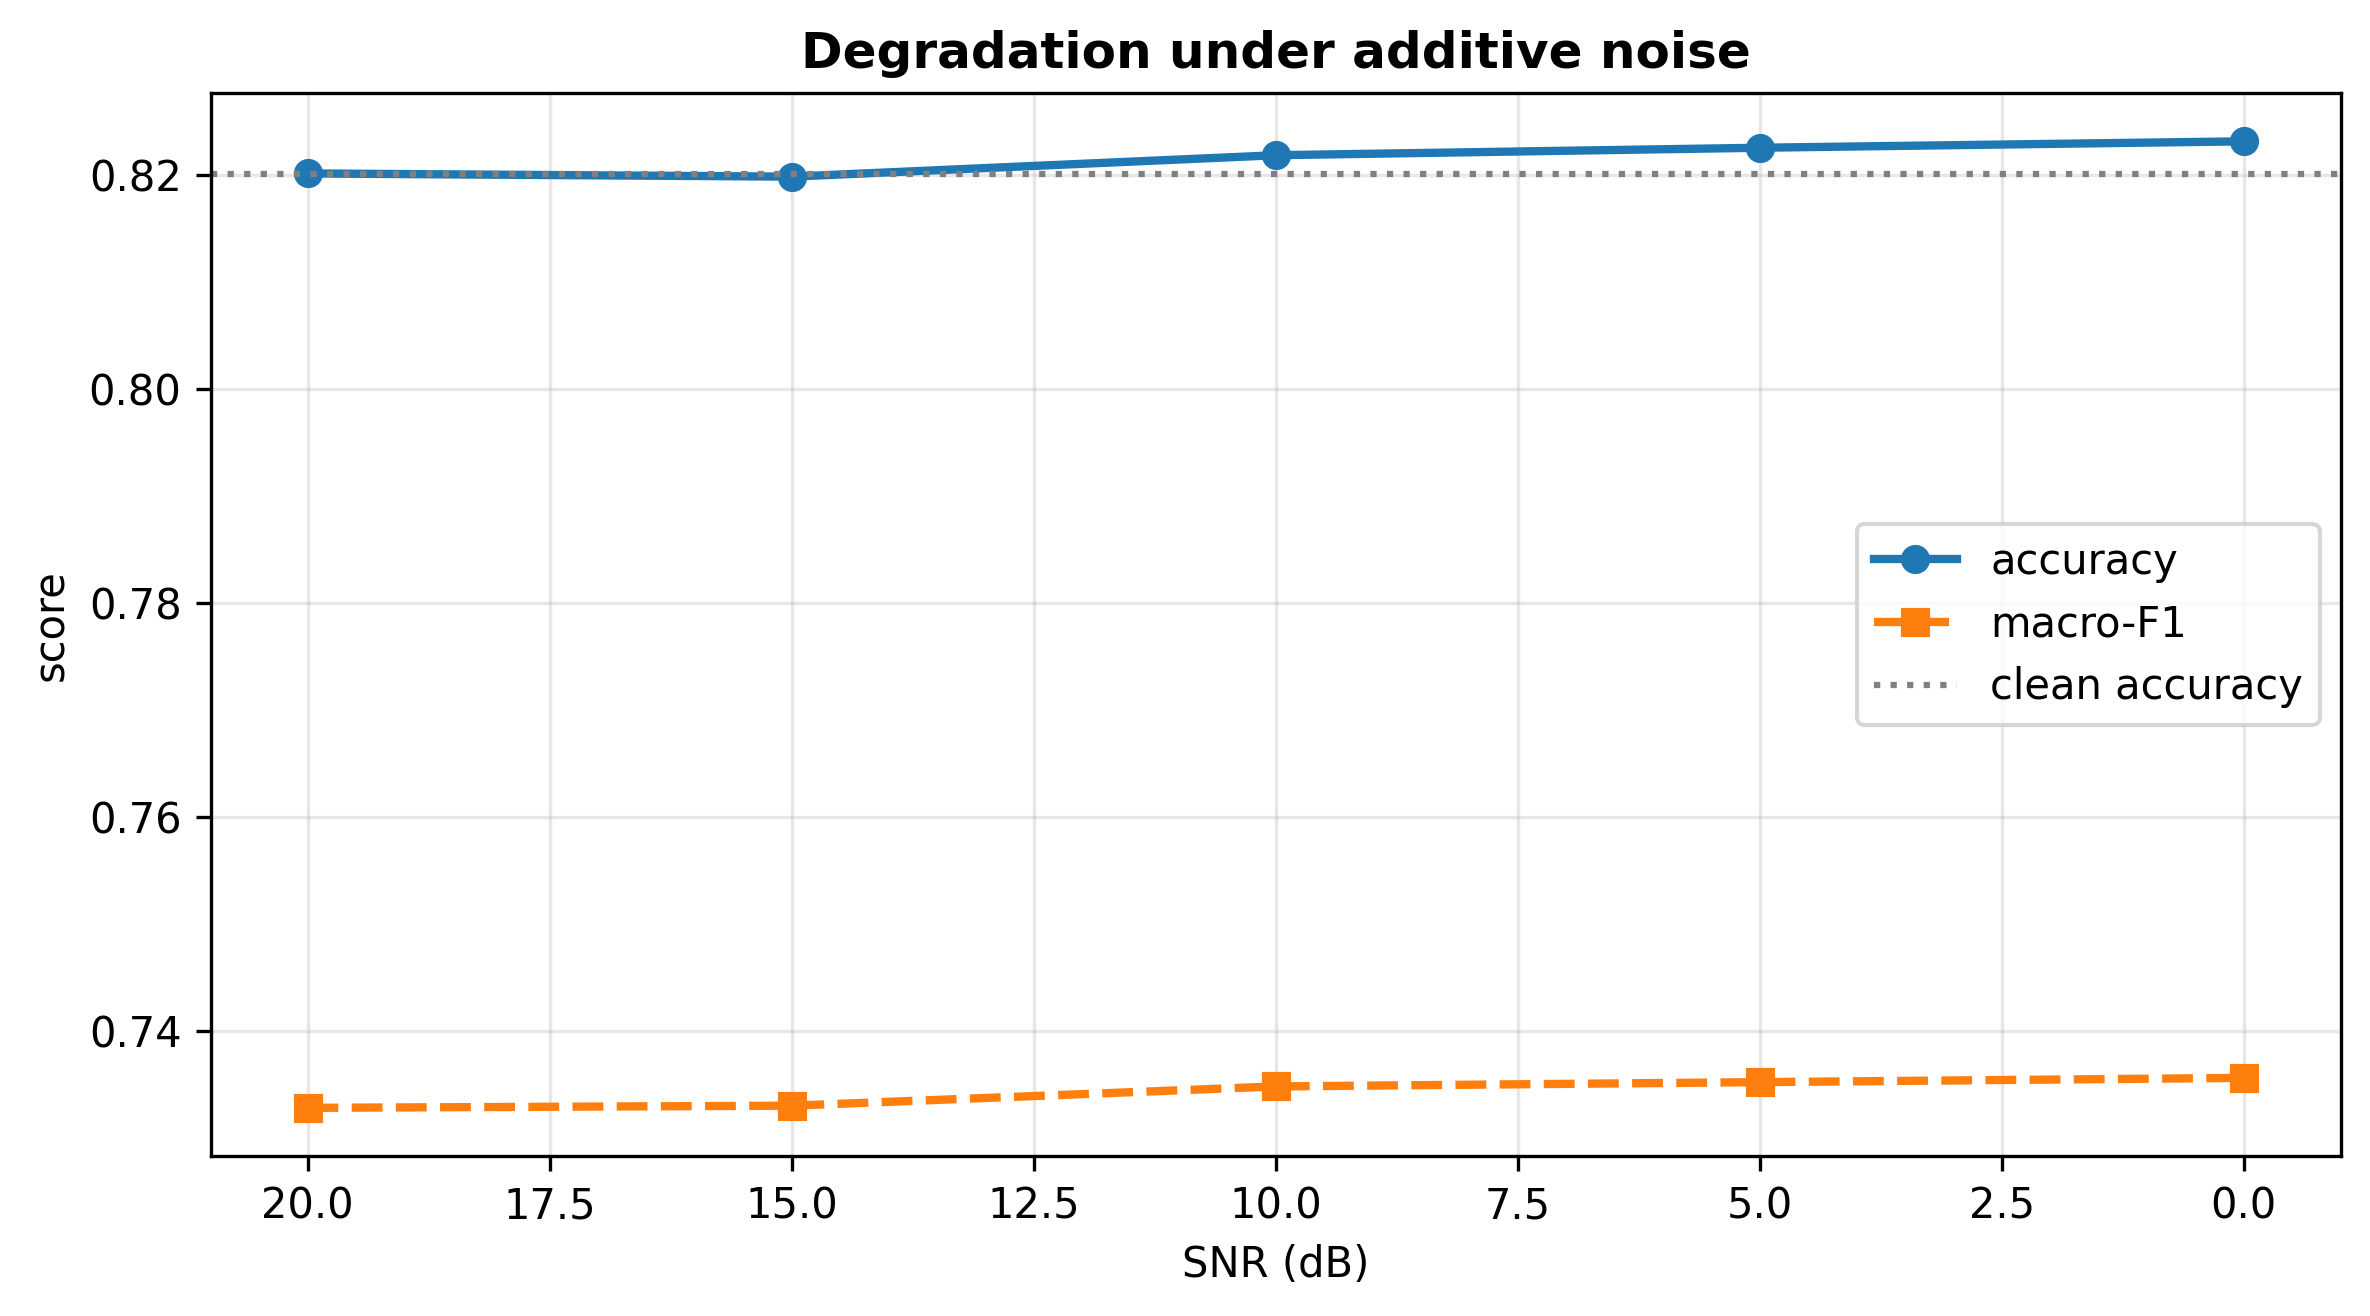
\includegraphics[width=0.95\linewidth]{figures/Inter_Patient/06_robustness.png}
\caption{Accuracy and macro-$F_1$ as a function of corruption severity, spanning the full range of Gaussian-noise and baseline-wander levels tested}
\label{fig:robust}
\end{figure}

The robustness result in Table~\ref{tab:robust} requires careful reading
rather than celebration. Across the whole 20~dB range of Gaussian noise,
accuracy changes by less than 0.004 and in fact drifts slightly upward as
the signal-to-noise ratio falls, and quadrupling the baseline-wander
amplitude leaves both metrics equally flat. A flat-to-slightly-positive
trend under added noise is a recognised artefact of band-limited pipelines:
the preprocessing band-pass suppresses much of the injected high-frequency
noise, and the residual noise acts as a mild regulariser on the decision
boundaries rather than as a corrupting influence. The practical conclusion
is nevertheless reassuring: the low-frequency morphological features (the
gross shape of the QRS complex and the template similarities) carry the
classification, and those are exactly the features that additive
high-frequency noise and slow baseline drift do not corrupt. For ambulatory
applications this is a desirable property, because such corruptions are the
rule rather than the exception. It should not be over-read, however: the
trend indicates primarily that this synthetic corruption model does not
engage the classifier's true failure modes, and robustness to synthetic
corruption is not equal to validation on a truly separate ambulatory
database, which remains future work.

\subsection{Provenance Controls}
\label{subsec:provenance}

Since the normal beats were drawn from two databases (MIT-BIH and NSR),
there is a potential for the classifier to learn a database ``fingerprint''
instead of cardiac morphology. A probe machine trained to predict the
source database achieved 0.8791 accuracy on distinguishing MIT-BIH from
NSR normal beats against a majority baseline of 0.8611, confirming that
such a short cut is available and is the main reason the CHF-derived
category was excluded from the five-class label space. To confirm that the five-class
results are not driven by this artefact, the test signals were
bandwidth-equalised: overall accuracy changed from 0.8200 to 0.8201, and
every per-class $F_1$ moved by at most 0.0004. This negligible change
indicates that the five-class AAMI performance is genuine cardiac
morphology, not a band-limiting database signature.

\subsection{Microcontroller Deployment}
\label{subsec:mcu}

Table~\ref{tab:mcu} reports the INT8-quantised deployment model, including
its accuracy, footprint, and measured latency.

\begin{table}[!t]
\centering
\caption[Deployment characteristics of the INT8-quantised tiny MCU model]{Deployment characteristics of the INT8-quantised tiny MCU model against the float32 MCU and full hybrid references (inter-patient protocol; latency measured on a Kaggle host, not on-device)}
\label{tab:mcu}
\begin{tabular}{lrrr}
\toprule
\textbf{Property} & \textbf{Hybrid (float32)} & \textbf{MCU float32} & \textbf{MCU INT8} \\
\midrule
Parameters       & 572{,}358 & 11{,}685 & 11{,}685 \\
Model size       & $\sim$6.8\,MB & 224\,KB & 29.9\,KB \\
Test accuracy    & 0.8200 & 0.6699 & 0.6746 \\
Latency (per beat) & 95.27\,ms & -- & 0.07\,ms \\
Peak tensor RAM  & -- & -- & 5.6\,KB \\
\bottomrule
\end{tabular}
\end{table}

Table~\ref{tab:mcu} shows the quantisation result, closing the deployment
loop for the microcontroller. Post-training INT8 quantisation not only
maintained but slightly enhanced accuracy (a ``quantisation cost'' of
$-0.0047$), and the resulting 29.9~KB flatbuffer uses only operators
supported by TFLite Micro, with no custom kernels. The measured per-beat
latency of 0.07~ms on the host is more than three orders of magnitude below
the 333~ms budget of a 3-beat/s arrhythmia stream, and the peak 5.6~KB
single-tensor working set fits easily in the SRAM of a modern Cortex-M
device. The standalone accuracy of this tiny network (0.6746) is far below
MSFT-Net's, and it corresponds to a size/accuracy operating point for the
most constrained targets rather than the full-accuracy path.

To fill the remaining gap (host-measured latency versus true on-device
runtimes), the INT8-quantised \emph{headline} MSFT-Net classifier was
flashed onto an STM32 microcontroller, and its footprint, memory usage, and
timing were measured directly. Table~\ref{tab:stm32} reports the on-device
results.

\begin{table}[!t]
\centering
\caption{On-device deployment characteristics of the INT8-quantised MSFT-Net on an STM32 microcontroller (128\,KB RAM, 512\,KB flash)}
\label{tab:stm32}
\begin{tabular}{lr}
\toprule
\textbf{Property} & \textbf{Value} \\
\midrule
Model (flash) size        & 288.16\,KB \\
Flash utilisation         & 56.28\% (of 512\,KB) \\
Total RAM usage           & 99{,}580\,B (75.97\% of 128\,KB) \\
AI activation memory      & 68.27\,KB \\
CPU cycles per inference  & 33{,}310{,}368 \\
Inference latency (per beat) & 185.057\,ms \\
Power draw                & 2.6\,W \\
\bottomrule
\end{tabular}
\end{table}

The on-device result in Table~\ref{tab:stm32} answers the qualification
raised for the tiny MCU model: real-time operation is confirmed on actually
measured target hardware rather than inferred from a host benchmark. The
per-beat latency of 185.057~ms is within the 333~ms budget of a 3-beat/s
arrhythmia stream, with a headroom of about 148~ms per beat. The 288.16~KB
flatbuffer occupies 56.28\% of the STM32's 512~KB flash, and the runtime
footprint (99{,}580 bytes of RAM in total, comprising the 68.27~KB
activation arena together with data and bss) consumes 75.97\% of the
device's 128~KB RAM, leaving a rather
restricted margin for application-level buffering such as signal
acquisition or communication stacks. The power drawn during an inference
was 2.6~W. This is a full-accuracy deployment of MSFT-Net (not the
intentionally downsized MCU variant of Table~\ref{tab:mcu}), and the
highlighted inter-patient accuracy of 0.8945 is achieved on-device at the
price of the larger footprint. The two deployment points of Tables
\ref{tab:mcu} and~\ref{tab:stm32} span the accuracy--footprint compromise a
practitioner can make: the tiny model is validated for the most
memory-constrained wearables, while the STM32-validated MSFT-Net serves
whenever full accuracy is required. In both instances the results prove
that the pipeline does not need to be a cloud service: real-time,
on-device, robust arrhythmia classification is achievable on
microcontroller hardware, the critical precondition for wearable
deployment.


\section{Cross-Protocol Synthesis}
\label{sec:crossprotocol}

The most critical analysis of this work is the side-by-side placement of
the two studies in this section. They use the same family of architectures
and the same core databases; the only change is the evaluation protocol.
Under the intra-patient protocol the model reaches 0.9859 accuracy and
0.9684 macro-$F_1$, while under the inter-patient protocol the same family
drops to 0.8945 accuracy and 0.8725 macro-$F_1$, a gap of roughly nine
points in accuracy and nearly ten in macro-$F_1$. Three strands of
continuity emerge from this comparison, and together they constitute the
substantive contribution of this work.

First, the headline number is an evaluation protocol. An ``intra-patient
result'' is not a better type of model; it is the same model measured on a
less difficult problem, in which the classifier has seen the typical
morphology of each test patient during training. Any comparison of
arrhythmia classifiers that does not control the protocol compares protocols
as well as models, and the nine-point gap quantifies exactly how large that
confound can be.

Second, the protocol alters the architectural conclusion, not just the
score. The BiLSTM is load-bearing under the intra-patient split
(Table~\ref{tab:intra_ablation}: $+0.0044$ accuracy) but not beneficial
under the inter-patient split (Table~\ref{tab:ablation}:
$\Delta\text{macro-}F_1 = +0.0194$ on removal). A practitioner who tuned
their architecture on an intra-patient split would ship a bigger, recurrent
model that performs worse on unseen patients; the failure mode that
motivates the compact MSFT-Net happens to be slightly worse on paper under
the permissive protocol.

Third, the fusion class is an invariant difficulty. It is the hardest class
under both protocols ($0.84$--$0.85$ $F_1$), which localises the one
remaining scientific challenge in beat morphology rather than in the
evaluation setup. The dedicated fusion pipeline of
Section~\ref{subsec:fbeat} is therefore a prerequisite for further
progress on $F$ beats.


\section{Summary of Findings}
\label{sec:summary}

Collectively, the two studies argue for a specific and limited set of
claims. Under the inter-patient protocol, the compact MSFT-Net attains
0.8945 accuracy and 0.8725 macro-$F_1$ with 167{,}090 parameters,
significantly outperforming a 3.4$\times$ larger
CNN--BiLSTM--Attention hybrid ($p \approx 0$), and the ablation identifies
the auxiliary feature vector, not the recurrent architecture, as the source
of performance. The targeted fusion-beat pipeline raises $F$ precision from
0.6000 to 0.8042 through hard-negative mining rather than augmentation; the
model is robust to ambulatory noise and baseline wander; its five-class
performance is shown not to be a database artefact; and it compresses to a
29.9~KB INT8 artefact whose accuracy was determined, not estimated. Under
the permissive intra-patient protocol, the same architecture family
reaches 0.9859 accuracy and 0.9684 macro-$F_1$ on a larger six-category
problem, but, as the cross-protocol synthesis of
Section~\ref{sec:crossprotocol} shows, that greater value comes from an
easier evaluation regime and a recurrent stage that actively hurts
inter-patient generalisation. The results avoid claiming external
validation beyond the databases used; real-time operation on target
hardware, calibrated probabilities with abstention, and faithful attribution
maps are indicated as future work rather than claimed, and the two-protocol
reporting is provided exactly to spread the claims that \emph{are} made to
their actual source.